\chapter{Problemas de vibração livre com o Método dos Elementos Virtuais}

\indent Neste capítulo, são analisados quatro problemas de vibração livre no estado plano:

    \begin{itemize}
        \item Uma chapa engastada no estado plano de tensões;
        \item Uma chapa engastada com furo circular no centro no estado plano de tensões;
        \item uma barragem de terra no estado plano de deformações, e
        \item uma parede estrutural de 4 pavimentos no estado plano de tensões. 
    \end{itemize}

\indent Todos os resultados aqui obtidos pelo MEV são comparados aos do MEF e aos do MEFG. Todas as três são técnicas numéricas que particionam o domínio em elementos e aproximam a solução localmente construindo sistemas de equações lineares. A principal diferença entre as técnicas é a maneira de construção da aproximação local.\\
\indent O MEF subdivide o espaço em elementos geométricos simples ou padronizados, como triângulos e retângulos. A aproximação da solução é feita unicamente com funções polinomiais, com a acurácia da solução dependendo do grau polinomial e da quantidade de elementos. Essa característica permite o mapeamento de todos os elementos através do uso de funções de forma, e a integração das matrizes de rigidez e massa pode ser feita diretamente através da quadratura de Gauss ou analiticamente para o caso de famílias de elementos não paramétricas. Porém, devido à limitação em relação aos tipos de elementos, a construção da malha deve ser rigorosa para não existir elementos muito distorcidos, com ângulos muito obtusos ou mal formados, pois estes degradam severamente a precisão da solução numérica.\\
\indent O MEFG é uma evolução do MEF utilizando a técnica de partição da unidade para enriquecer o espaço de aproximação. Enquanto a base do MEF é mantida, o MEFG multiplica as funções de forma por funções de enriquecimento que refletem o comportamento físico esperado do problema. Problemas abordados através do MEFG ganham graus de liberdade adicionais nos nós correspondentes aos modos de enriquecimento. As integrais são mais complexas e frequentemente exigem esquemas de integração numérica adaptativa ou mais refinados devido à aplicação de funções não polinomiais.\\
\indent Para a comparação dos resultados do MEV com resultados de referência obtidos pelo MEF e o MEFG desenvolvidos no capítulo 5 são
utilizadas as seguintes métricas
    \begin{enumerate}
        \item O erro médio absoluto (MAE)
        \item Erro percentual médio absoluto (MAPE) das frequências naturais para cada modo de vibração;
        \item Média da raiz erro ao quadrado normalizado (NRMSE)
        \item A média geométrica do erro (MG)
        \item Coeficiente de acurácia de discretização (CAD)
        \item Ganho de precisão relativo (GPR)
        \item Capacidade de aproximação (CA)
    \end{enumerate}
    
\indent O erro relativo das frequências naturais para cada modo de vibração é calculado por:

\begin{equation}
    e_{\mathrm{rel}} = \left| \frac{\omega - \tilde{\omega}}{\omega} \right|,
    \label{eq:1.1}
\end{equation}

\noindent com $\omega$ sendo a frequência de referência e $\tilde{\omega}$ a frequência obtida pelo MEV. Para a avaliação de um desempenho médio representativo dos dados utiliza-se a média do erro relativo percentual (MAPE), utilizado no trabalho de \citet{custodio2022metodo} e de \citet{torii2012analise} e sendo uma das médias mais comuns em diversos trabalhos. Para cada malha, a MAPE é medida pelo quociente entre a soma dos erros absolutos e a quantidade de modos analisados:	

\begin{equation}
    e_{\mathrm{MAPE}} = \frac{\sum_{i=1}^{n_{\mathrm{modos}}} e_{\mathrm{rel},i} }{n_{\mathrm{modos}}}.
    \label{eq:1.2}
\end{equation}

\indent A média absoluta não pondera os resultados das frequências, de tal forma que um modo que possua um erro absoluto alto seja desconsiderado por outro modo com erro absoluto ótimo. Destarte, para estudo da eficiência global das malhas, será utilizado a raiz do erro quadrático médio (NRMSE):

\begin{equation}
    e_{\mathrm{NRMSE}} = \sqrt{\frac{\sum_{i=1}^{n_{\mathrm{modos}}} (\omega_i - \tilde{\omega}_i)^2}{\sum_{i=1}^{n_{\mathrm{modos}}} (\omega_i)^2 }}. 
    \label{eq:1.3}
\end{equation}

\indent A NRMSE é uma métrica de erro baseada na norma $L^2$, Eq.~\ref{eq:4.9}, representando a relação entre da "energia do erro" em relação a "energia global" da grandeza analisada. Por elevar os erros ao quadrado, a NRMSE garante uma penalização muito maior do que a da MAPE, o que o torna ideal para visualização dos resultados de maneira global.\\
\indent Tendo dois parâmetros de erro, propõem a utilização da média geométrica (MG) para unificação das médias dos erros como índice comparativo dos erros calculados como um índice composto:

\begin{equation}
    e_{\mathrm{MG}} = \sqrt{e_{\mathrm{NRMSE}} \, e_{\mathrm{MAPE}}}.
    \label{eq:1.4}
\end{equation}

A escolha da média geométrica para índice composto é porque ela permite a união de dois parâmetros sem que um domine o outro.\\
\indent A MAPE trata todos os dados de maneira idêntica, onde um resultado bom ou ruim pode afetar o valor final. O desvio padrão permite identificar a variação de um conjunto de dados com relação à média. Aplicando-o ao cálculo do erro percentual de modo de vibração, mede-se a regularidade dos erros por modo de vibração em uma malha. Para um estudo da sensibilidade ao refino da malha, introduz-se a média absoluta do desvio padrão (MASD): 

\begin{equation}
    e_{MASD,grossa} = \frac{1}{n_{malhas}} \sum_{j=1}^{n_{malhas}} \left(\sqrt{\frac{\sum_{i=1}^{n_{modos}}(e_{rel,i} - e_{MAPE,j})^2}{n_{modos}-1}} \right).
    \label{eq:1.a1}
\end{equation}

\indent Para mediação do erro entre a malha mais grossa e a malha mais refinada serão utilizadas a queda absoluta por peso percentual (QA), o fator de redução (FR) e o ganho de precisão (GP). Esses valores são utilizados na avaliação dos resultados da MAPE:

\begin{equation}
    QA = e_{MAPE,grossa} - e_{MAPE,refinada},
    \label{eq:1.a2}
\end{equation}

\begin{equation}
    FR = \frac{e_{MASD,grossa}}{e_{MASD,refinada}} \quad \text{e}
    \label{eq:1.a3}
\end{equation}

\begin{equation}
    GP = \frac{e_{MAPE,grossa} - e_{MAPE,refinada}}{e_{MAPE,grossa}}
    \label{eq:1.a4}
\end{equation}

\indent O coeficiente de acurácia de discretização (CAD) mede a evolução de uma malha conforme discretizada tomando como base a malha mais grossa, que possui menor custo computacional, para a malha mais refinada de maior custo. O parâmetro serve de indicativo para qual malha o refino $h$ atinge um teto de aproximação. O parâmetro é calculado por:

\begin{equation}
    CAD = \frac{\text{e}_{MG,\text{grossa}} - \text{e}_{MG,\text{atual}}}{\text{e}_{MG,\text{grossa}} - \text{e}_{MG,\text{refinada}}}.
    \label{eq:1.5}
\end{equation}

\indent Outra relação do CAD está relacionada ao ganho de acurácia em relação à malha mais grossa e de maneira inversa a malha mais refinada. Para o cálculo do CAD será utilizada a média geométrica como base.\\
\indent Visando à comparação entre métodos, um índice similar ao CAD é proposto, o ganho de precisão relativo (GPR). Esse índice mede a melhora de precisão entre dois métodos numéricos e um terceiro resultado de referência -- Numérico ou a solução exata. O índice é calculado como:

\begin{equation}
    GPR = \frac{\text{e}_{MG,\text{MEF}} - \text{e}_{MG,\text{MEV}}}{\text{e}_{MG,\text{MEF}}}.
    \label{eq:1.6}
\end{equation}

\indent O último parâmetro de estudo é baseado no índice CA elaborado por (\citet{cittadin2020enriquecimento}). Em seu uso original esse parâmetro mede as diferenças de
aproximação entre duas formulações com enriquecimento de funções e uma referência de base para estimativa de acurácia. O índice foi adaptado 
de modo que se possa comparar a diferença dos erros de duas técnicas numéricas em relação a uma terceira de referência. Este índice será 
utilizado neste trabalho para comparação do ganho de precisão entre o MEV e o MEFG em relação ao MEF clássico.

\begin{equation}
    CA = \frac{\text{e}_{MG,\text{MEF}} - \text{e}_{MG,\text{MEV}}}{\text{e}_{MG,\text{MEF}} - \text{e}_{MG,\text{MEFG}}}.
    \label{eq:1.7}
\end{equation}

\indent A avaliação dos resultados do CA segue:

\begin{enumerate}
    \item $CA < 0$: O MEV apresenta maior erro do que o MEF tradicional.
    \item $0 < CA < 1$: O MEV é mais preciso que o MEF, porém menos do que o MEFG.
    \item $CA = 1$: O MEV possui a mesma precisão do MEFG.
    \item $CA > 1$: O MEV supera tanto o MEF quanto o MEFG em precisão.
\end{enumerate}

\indent Neste trabalho a formulação do MEV e outras rotinas computacionais são implementadas com um solver programado em Modern Fortran
e o Gnuplot para visualização de resultados. Gráficos e tabelas comparativas são feitas com auxílio do Google planilhas. As malhas são gerados com o uso do software AutoCAD.\\

\textbf{\underline{Esclarecimentos ao leitor:}}\\

\indent Como os elementos virtuais podem possuir arestas com 180° entre si, podem existir malhas com a mesma quantidade de elementos, mas com diferentes quantidades de nós. Assim, adota-se o seguinte padrão de nomenclatura para as malhas utilizadas daqui em diante neste trabalho: $$XX\#\#\#N\#\#\#k\#$$. 

    \begin{itemize}
        \item X - Letras
        \item \# - Números
    \end{itemize}
    
\indent O primeiro conjunto de letras corresponde às iniciais do problema. O primeiro conjunto de números representa a quantidade de elementos na malha. N\#\#\# é a quantidade de nós. k\# é o grau polinomial que aqui varia de 1 a 2. Exemplo: PF32N74k1 $\rightarrow$ Placa com furo de 32 elementos, 74 nós e aproximação de primeira ordem. \\
\indent Todos os problemas aqui tratados são de natureza vetorial, assim a quantidade de graus de liberdade por elemento equivale a duas vezes a quantidade de nós. Em aproximações de segunda ordem, haverá dois graus de liberdade internos adicionais aos dos nós relativos a vetorização dos momentos internos para $k=2$. 

\section{Chapa engastada}

\indent Para o problema da chapa engastada (Figura~\ref{fig:5.1.1}) são executados estudos do comportamento das técnicas de estabilização apresentadas no Capítulo~\ref{cap:4} em relação ao refino de uma malha uniforme, do efeito da distorção da geometria dos elementos no erro da solução e uma comparação dos resultados obtidos com o MEFG e o método dos elementos finitos hierárquicos desenvolvidos por \citet{torii2012analise}.

\begin{figure}[H]
    \centering
    \caption{Geometria e condições de contorno do problema da chapa engastada.}
    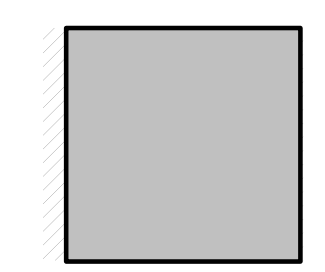
\includegraphics[width=0.4\textwidth]{figuras/Capítulo 5/Placa quadrada/Placa engastada.png}
    \label{fig:5.1.1}

    {\small \textbf{Fonte:} \citet{torii2012analise}.}
\end{figure}

\indent As propriedades materiais da chapa são: módulo de elasticidade $E = 2,1 \cdot 10^{11} \, \left(\frac{N}{m^2}\right)$, coeficiente de Poisson $\nu = 0,3$ e massa específica $\rho = 8000 \, \left(\frac{kg}{m^3}\right)$. A chapa apresenta dimensões de $1,0\,(m)$ e espessura $d = 0,05\,(m)$. Os movimentos na borda esquerda estão impedidos.

\indent Utilizando os resultados de referência de \citet{torii2012analise}, obtidos com o MEFH polinomial em uma malha $4\times4$ de elementos finitos de ordem igual a 9, compara-se o comportamento do seguinte grupo de estabilizações em relação ao refino da malha:
\begin{enumerate}
    \item Equação~\ref{eq:4.67} com fator de escala físico;
    \item Equação~\ref{eq:4.67} com fator de escala uniforme;
    \item Equação~\ref{eq:4.67} com fator de escala D-Recipe híbrido;
    \item Equação~\ref{eq:4.68} com fator de escala equivalente ao traço calibrado da parcela de consistência;
    \item Equação~\ref{eq:4.67} com fator de escala D-Recipe.
\end{enumerate}

\indent Para o estudo do efeito da estabilização sob o refino da malha serão utilizadas três malhas com elementos quadrilaterais uniformes: CU4N9k1, CU16N25k1 e CU64N81k1. Observando a Figura~\ref{subfig:5.1.2a}, percebe-se um comportamento similar entre as malhas, com os maiores erros concentrados nas frequências intermediárias. Ao se refinar a malha para 25 e 64 elementos (Figuras~\ref{subfig:5.1.2b} e \ref{subfig:5.1.2c}), os maiores erros, que antes se concentravam nas regiões intermediárias, deslocam-se para as frequências mais altas.

\begin{figure}[H]
    \centering
    \caption{Erro relativo em função do modo de vibração para as malhas CU4N9k1, CU16N25k1 e CU64N81k1.}
    \label{fig:5.1.2}
    \begin{subfigure}[b]{0.45\textwidth}
        \centering
        \caption{Malha de 4 elementos}
        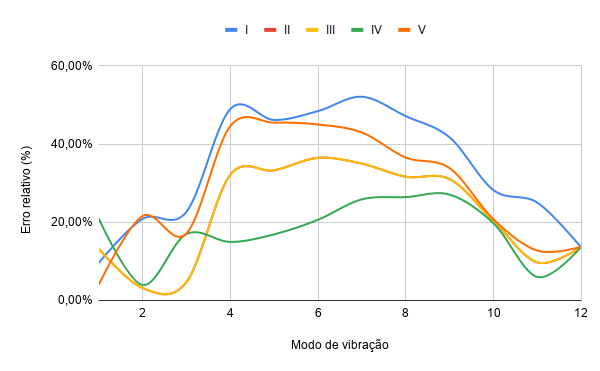
\includegraphics[width=\textwidth]{figuras/Capítulo 5/Placa quadrada/Erro absoluto x Modo de vibração (Malha de 4 elementos).png}
        \label{subfig:5.1.2a}
    \end{subfigure}
    \hfill
    \begin{subfigure}[b]{0.45\textwidth}
        \centering
        \caption{Malha de 16 elementos}
        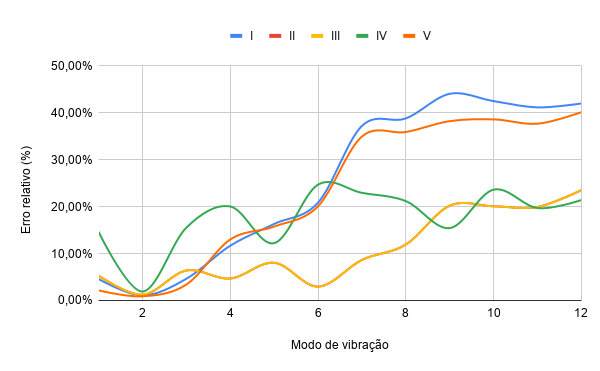
\includegraphics[width=\textwidth]{figuras/Capítulo 5/Placa quadrada/Erro absoluto x Modo de vibração (Malha de 16 elementos).png}
        \label{subfig:5.1.2b}
    \end{subfigure}

    \begin{subfigure}[b]{0.45\textwidth}
        \centering
        \caption{Malha de 64 elementos}
        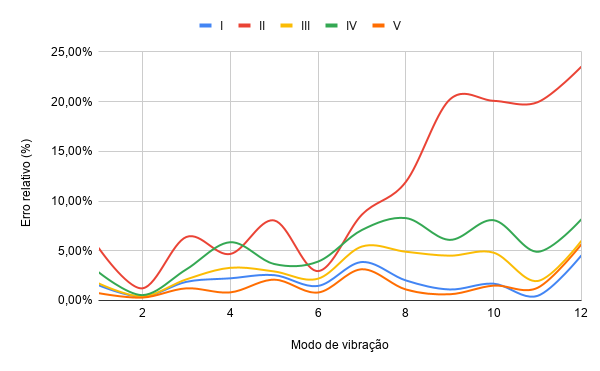
\includegraphics[width=\textwidth]{figuras/Capítulo 5/Placa quadrada/Erro absoluto x Modo de vibração (Malha de 64 elementos).png}
        \label{subfig:5.1.2c}
    \end{subfigure}

    {\small \textbf{Fonte:} Elaborado pelo autor (2026).}
\end{figure}

\indent Fazendo uma observação global dos resultados da Figura~\ref{fig:5.1.3}, verifica-se que todas as estabilizações tendem a convergir com o refino $h$, porém não na mesma velocidade. Isso pode ser notado ao se comparar as estabilizações~\textrm{I} e~\textrm{IV}: a estabilização com menor erro em malhas grossas não apresenta o menor erro na malha mais refinada. Esse resultado indica que não há um método de estabilização ideal para todos os problemas e malhas.

\begin{figure}[H]
    \centering
    \caption{MAPE em função do refino da malha para as diferentes estabilizações.}
    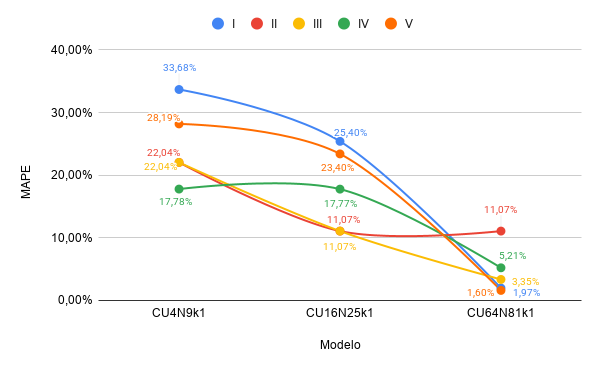
\includegraphics[width=\textwidth]{figuras/Capítulo 5/Placa quadrada/MAPE x Malha.png}
    \label{fig:5.1.3}

    {\small \textbf{Fonte:} Elaborado pelo autor (2026).}
\end{figure}

\begin{table}[htbp]
    \centering
    \caption{Métricas de desempenho das estabilizações sob refino de malha.}
    \label{tab:5.a.1}
    \small % Reduz o tamanho da fonte para o padrão de tabelas
    \begin{tabular}{lccccc}
        \toprule
        \textbf{Parâmetro} & \textbf{I} & \textbf{II} & \textbf{III} & \textbf{IV} & \textbf{V} \\
        \midrule
        QA (p.p) & 31,71\% & 10,96\% & 18,69\% & 12,57\% & 26,58\% \\
        FR       & 17,07   & 1,99    & 6,57    & 3,41    & 17,61   \\
        GP       & 94,14\% & 32,55\% & 55,48\% & 37,32\% & 78,93\% \\
        MASD     & 11\%    & 9\%     & 7\%     & 5\%     & 11\%    \\
        \bottomrule
    \end{tabular}
    
    \vspace{0.2cm}
    \raggedright
    \textbf{Fonte:} Elaborado pelo autor (2026).
\end{table}

\indent As estabilizações~\textrm{I} e~\textrm{V} demonstraram-se as mais sensíveis ao refino da malha, com quedas absolutas de $31,71\%$ e $26,58\%$ (Tabela~\ref{tab:5.a.1}), obtendo os menores erros na malha mais refinada. Uma peculiaridade é que, enquanto a estabilização~\textrm{I} depende apenas da física do problema, a estabilização~\textrm{V} é baseada unicamente na matriz de consistência, ou seja, trata-se de uma estabilização puramente geométrica.\\
\indent As estabilizações~\textrm{II} e~\textrm{III} obtiveram resultados idênticos, apesar de a estabilização~\textrm{II} deixar de convergir para a solução de referência a partir da malha de 25 elementos. Em contraste com a estabilização~\textrm{II}, a estabilização~\textrm{IV} só começa a apresentar queda do erro de solução a partir da malha de 25 elementos. Observando a Figura~\ref{fig:5.1.2}, nota-se que, para a estabilização~\textrm{IV}, existe uma redistribuição dos erros dos modos de vibração entre as malhas de 4 e 25 elementos.\\
\indent Foi adotada a estabilização~\textrm{IV} como formulação de referência do MEV para as análises subsequentes, mantendo-se inalterados o tipo de estabilização e seu fator multiplicativo entre os diferentes problemas. A escolha teve como principal critério a obtenção de um comportamento de convergência uniforme e robusto (como pode ser verificado pela MASD na Tabela~\ref{tab:5.a.1}), evitando que a comparação com o MEF e o MEFG fosse condicionada por uma calibração específica para cada problema. Para a estabilização da matriz de massa será utilizada a área do elemento.\\
\indent O estudo do impacto da distorção foi realizado para as malhas da Figura~\ref{fig:5.1.4}. As frequências obtidas, juntamente com os valores de \citet{torii2012analise} utilizados como referência comparativa, estão documentadas na Tabela~\ref{tab:5.a.2}.

\begin{figure}[H]
    \centering
    \caption{Malhas utilizadas no estudo de distorção.}
    \label{fig:5.1.4}
    \begin{subfigure}[b]{0.3\textwidth}
        \centering
        \caption{Malha uniforme}
        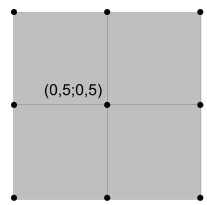
\includegraphics[width=\textwidth]{figuras/Capítulo 5/Placa quadrada/malha uniforme.png}
        \label{subfig:5.1.4a}
    \end{subfigure}
    \hfill
    \begin{subfigure}[b]{0.3\textwidth}
        \centering
        \caption{Malha distorcida}
        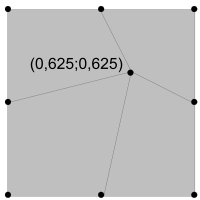
\includegraphics[width=\textwidth]{figuras/Capítulo 5/Placa quadrada/malha distorcida.png}
        \label{subfig:5.1.4b}
    \end{subfigure}
    \hfill
    \begin{subfigure}[b]{0.3\textwidth}
        \centering
        \caption{Malha muito distorcida}
        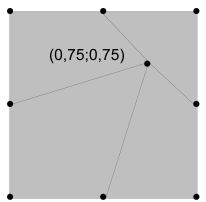
\includegraphics[width=\textwidth]{figuras/Capítulo 5/Placa quadrada/Malha muito distorcida.png}
        \label{subfig:5.1.4c}
    \end{subfigure}

    {\small \textbf{Fonte:} \citet{torii2012analise}.}
\end{figure}

\begin{table}[htbp]
    \centering
    \caption{Frequências naturais (rad/s).}
    \label{tab:5.a.2}
    \small % Reduz o tamanho da fonte para caber melhor na página
    \begin{tabular}{lcccccc}
        \toprule
        \textbf{MODO} & \textbf{REFERÊNCIA} & \textbf{CU4N9k1} & \textbf{CU16N25k1} & \textbf{CU64N81k1} & \textbf{CD4N9k1} & \textbf{CSD4N9k1} \\
        \midrule
        1  & 3372,13 & 4082,522  & 3866,005  & 3468,057  & 4488,16  & 4524,89  \\
        2  & 8092,72 & 8412,942  & 8246,607  & 8136,102  & 8439,55  & 8495,58  \\
        3  & 9079,09 & 10620,337 & 10488,012 & 9363,019  & 12698,50 & 13414,50 \\
        4  & 14427,23 & 12267,837 & 17317,711 & 15272,151 & 16915,09 & 16773,58 \\
        5  & 15558,23 & 12927,268 & 17457,232 & 16128,64  & 17482,00 & 17409,24 \\
        6  & 16511,96 & 13101,489 & 20589,566 & 17157,246 & 19430,52 & 18372,58 \\
        7  & 20812,77 & 15427,396 & 25586,194 & 22288,364 & 19758,28 & 18931,15 \\
        8  & 21911,61 & 16119,742 & 26551,84  & 23726,551 & 20064,89 & 19751,92 \\
        9  & 24194,74 & 17648,211 & 27927,119 & 25669,076 & 21384,09 & 21871,51 \\
        10 & 24349,42 & 19552,591 & 30102,516 & 26314,775 & 22885,75 & 26243,93 \\
        11 & 25319,9  & 23802,009 & 30306,481 & 26559,417 & 28050,27 & 30692,84 \\
        12 & 26790,31 & 30485,903 & 32526,143 & 28980,314 & 34321,08 & 42673,69 \\
        \bottomrule
    \end{tabular}
    
    \vspace{0.2cm}
    \raggedright
    \textbf{Fonte:} Elaborado pelo autor (2026).
\end{table}

\indent Comparando o erro global da solução com diferentes malhas (Figura~\ref{fig:5.1.5}), verifica-se que, apesar de a distribuição dos nós em malhas com a mesma quantidade de elementos afetar o erro, o impacto é significativamente pequeno quando comparado ao aumento da quantidade de elementos.

\begin{figure}[H]
    \centering
    \caption{MAPE em função da malha: comparação entre refino e distorção.}
    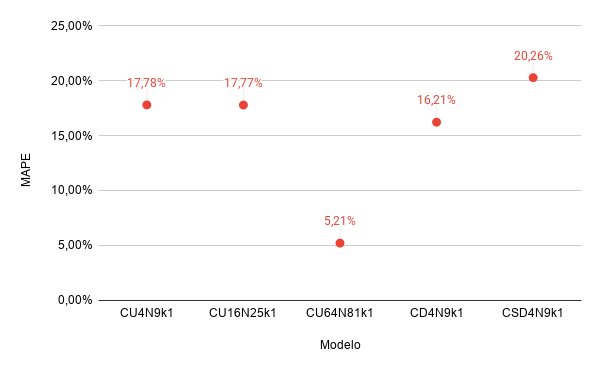
\includegraphics[width=\textwidth]{figuras/Capítulo 5/Placa quadrada/MAPE x Malha - Comparação de refino e distorção.png}
    \label{fig:5.1.5}

    {\small \textbf{Fonte:} Elaborado pelo autor (2026).}
\end{figure}

\indent Percebe-se que a malha distorcida apresentava um erro menor que a malha uniforme. Por isso, avalia-se o erro relativo em cada modo de vibração a fim de investigar a maneira como a topologia dos nós impacta o erro de cada modo. Avaliando a Figura~\ref{fig:5.1.6}, observa-se inicialmente que a malha uniforme demonstra um comportamento mais monotônico quando comparada às malhas distorcidas. Verifica-se, também, que os modos mais suscetíveis aos erros da topologia são os modos 3 e 12.

\begin{figure}[H]
    \centering
    \caption{Erro relativo em função do modo de vibração — estudo de distorção.}
    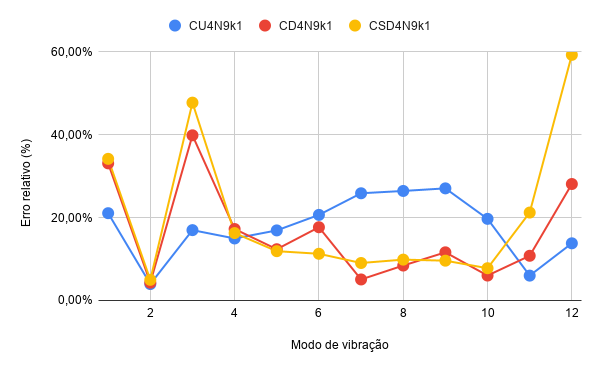
\includegraphics[width=\textwidth]{figuras/Capítulo 5/Placa quadrada/Erro relativo X Modo de vibração - Estudo de distorção.png}
    \label{fig:5.1.6}

    {\small \textbf{Fonte:} Elaborado pelo autor (2026).}
\end{figure}

\indent Calculando o desvio padrão da malha, chegam-se aos valores de $7,41\%$ para a malha uniforme, $11,62\%$ para a malha distorcida e $17,52\%$ para a malha severamente distorcida. Isso permite concluir que a topologia dos nós afeta drasticamente os erros dos diferentes modos de vibração. Também é possível concluir que o valor de erro inferior da malha distorcida trata-se de uma representação inadequada pelo MAPE. \\
\indent Para finalizar os estudos propostos neste problema, faz-se uma comparação dos erros obtidos pelo MEV com os do MEFG (com $\beta = \pi$ e $\beta = 3\pi/2$) e com o MEFH de ordem 5 de \citet{torii2012analise}, apresentados na Figura~\ref{fig:5.1.7}. Ao se utilizar uma mesma malha de 4 elementos, os resultados do MEV foram, em sua totalidade, inferiores aos do MEFG e do MEFH. Para a malha de elementos virtuais mais refinada, o MEV obteve respostas mais próximas da solução de referência apenas para os modos 1 e 2.

\begin{figure}[H]
    \centering
    \caption{Erro relativo em função do modo de vibração — comparação entre métodos.}
    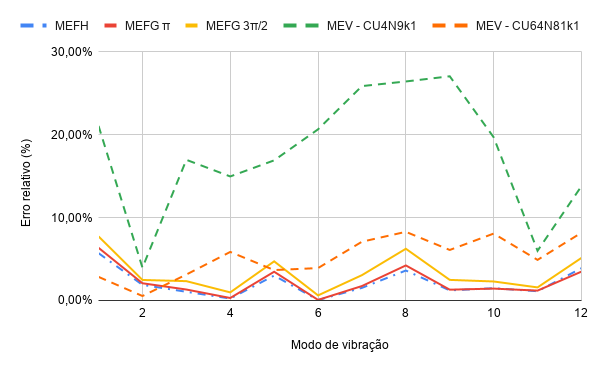
\includegraphics[width=\textwidth]{figuras/Capítulo 5/Placa quadrada/Erro relativo x Modo de vibração - Comparação entre métodos.png}
    \label{fig:5.1.7}

    {\small \textbf{Fonte:} Elaborado pelo autor (2026).}
\end{figure}

\indent A Figura~\ref{fig:5.9} apresenta as deformadas dos 4 primeiros modos de vibração:

\begin{figure}[H]
    \centering
    \caption{Deformadas dos 4 primeiros modos de vibração.}
    \label{fig:5.9}
    \begin{subfigure}[b]{0.45\textwidth}
        \centering
        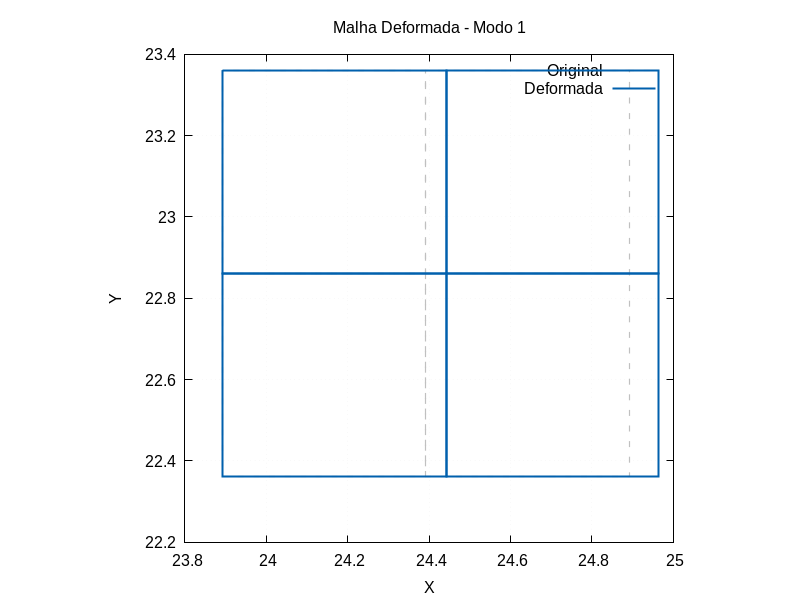
\includegraphics[width=\textwidth]{figuras/Capítulo 5/Placa quadrada/deformed_mode_1.png}
        \label{fig:5.9a}
    \end{subfigure}
    \hfill
    \begin{subfigure}[b]{0.45\textwidth}
        \centering
        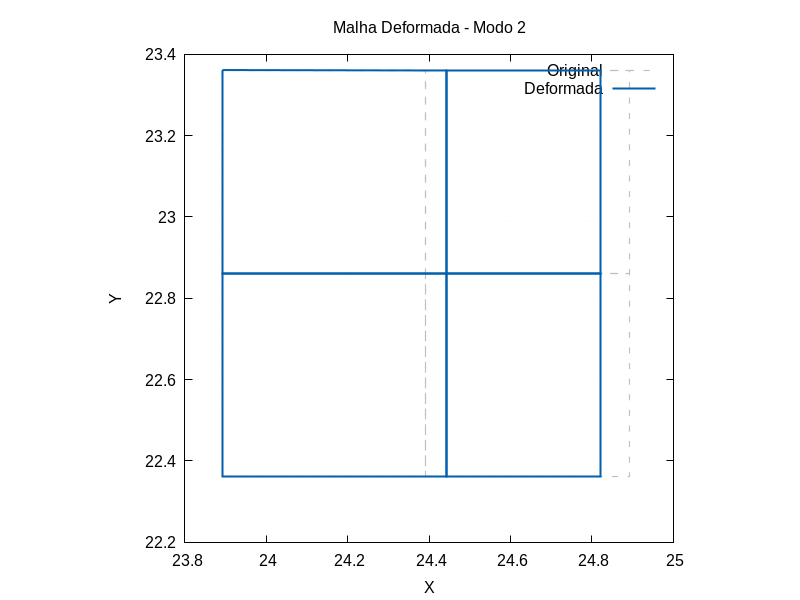
\includegraphics[width=\textwidth]{figuras/Capítulo 5/Placa quadrada/deformed_mode_2.png}
        \label{fig:5.9b}
    \end{subfigure}
    \vspace{3mm}
    \begin{subfigure}[b]{0.45\textwidth}
        \centering
        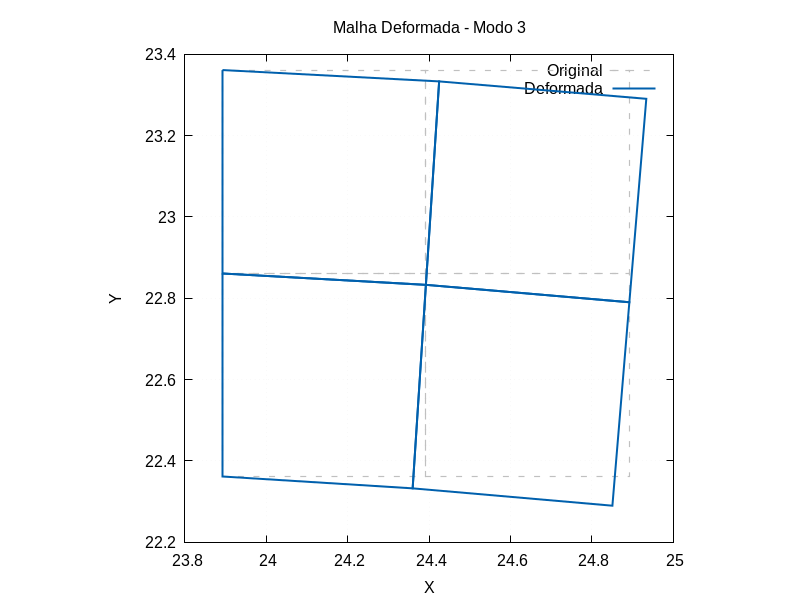
\includegraphics[width=\textwidth]{figuras/Capítulo 5/Placa quadrada/deformed_mode_3.png}
        \label{fig:5.9c}
    \end{subfigure}
    \hfill
    \begin{subfigure}[b]{0.45\textwidth}
        \centering
        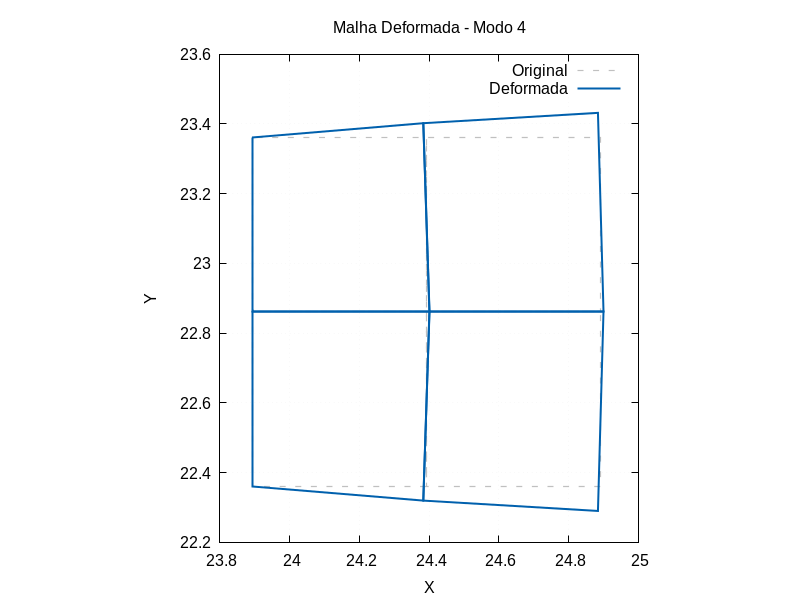
\includegraphics[width=\textwidth]{figuras/Capítulo 5/Placa quadrada/deformed_mode_4.png}
        \label{fig:5.9d}
    \end{subfigure}

    {\small \textbf{Fonte:} Elaborado pelo autor (2026).}
\end{figure}


\section{Chapa com furo circular}

\indent O segundo problema consiste em uma chapa engastada de espessura unitária com um furo no centro, apresentando módulo de elasticidade $E = 1\text{ (N/m}^2\text{)}$, densidade constante no elemento $\rho = 1\text{ (kg/m}^3\text{)}$ e coeficiente de Poisson $\nu = 0,3$. A geometria pode ser observada na Figura~\ref{fig:5.1}.

    \begin{figure}[H]
        \centering
        \caption{Geometria e condições de contorno do problema da chapa com furo circular.}
        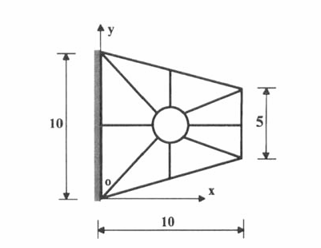
\includegraphics[width=0.7\textwidth]{figuras/Capítulo 5/Placa com furo/5.1.png}
        \label{fig:5.1}

        {\small \textbf{Fonte:} \citet{asymptoticsolutionspredictednaturalfrequenciestwodimensionalelasticsolidvibrationproblemsfiniteelementanalysis1996}.}
    \end{figure}

\indent O problema foi proposto inicialmente no trabalho de \citet{asymptoticsolutionspredictednaturalfrequenciestwodimensionalelasticsolidvibrationproblemsfiniteelementanalysis1996} utilizando o estado plano de tensões. A intenção dos autores foi a utilização de correção dos resultados do MEF com o uso de soluções assintóticas, que, segundo eles, possui solução mais precisa. O mesmo problema foi abordado por \citet{cittadin2020enriquecimento} como referência de desempenho para o MEFG. \\
\indent Para o problema da Figura~\ref{fig:5.1}, investiga-se o comportamento do MEV para uma malha fixa de 8 elementos, contudo utilizando diferentes quantidades de nós na fronteira dos elementos com o furo para simular o contorno circular, (Figura~\ref{fig:5.2}). 

    \begin{figure}[H]
        \centering
        \caption{Elementos de uma mesma malha com diferentes quantidades de nós. Observe que em a) o furo é modelado com apenas os dois nós de vértice e um nó interno, enquanto em b) há três nós internos modelando a geometria do furo. Estes nós foram adicionados sem alterar a ordem de interpolação polinomial.}
        \label{fig:5.2}
        \begin{subfigure}[b]{0.45\textwidth}
            \centering
            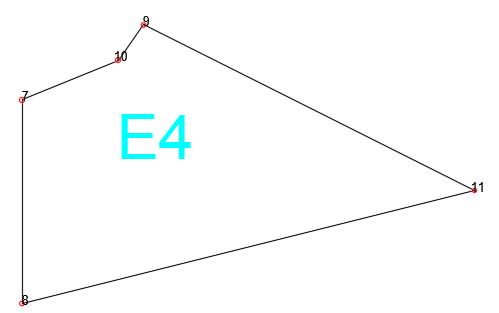
\includegraphics[width=0.8\textwidth]{figuras/Capítulo 5/Placa com furo/f1.png}
            \label{fig:5.2a}
        \end{subfigure}
        \hfill
        \begin{subfigure}[b]{0.45\textwidth}
            \centering
            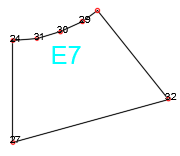
\includegraphics[width=0.7\textwidth]{figuras/Capítulo 5/Placa com furo/f2.png}
            \label{fig:5.2b}
        \end{subfigure}

        \centerline{{\small \textbf{Fonte:} Elaborado pelo autor (2026).}}
    \end{figure}  

\indent Comparam-se os valores das frequências naturais com as soluções do MEF com uma malha extremamente refinada, obtidas de \citet{asymptoticsolutionspredictednaturalfrequenciestwodimensionalelasticsolidvibrationproblemsfiniteelementanalysis1996}, o modelo de elementos finitos com correção assintótica de \citet{asymptoticsolutionspredictednaturalfrequenciestwodimensionalelasticsolidvibrationproblemsfiniteelementanalysis1996}, e o modelo de elementos finitos generalizados, com 480 graus de liberdade, de \citet{cittadin2020enriquecimento} para os primeiros dez modos de vibração. Os resultados se encontram resumidos na Tabela~\ref{tab:5.1}.

% Nota: Certifique-se de ter o pacote \usepackage{makecell} no preâmbulo do seu documento LaTeX.

\begin{table}[htbp]
    \centering
    \caption{Frequências naturais obtidas para os primeiros dez modos de vibração (rad/s) para malha de 8 elementos.}
    \label{tab:5.1}
    \small % Reduz o tamanho da fonte para manter a tabela compacta
    \begin{tabular}{lccccccc}
        \toprule
        \textbf{MODO} & \textbf{REF} & \makecell{\textbf{MEF}\\\textbf{(32 gl)}} & \makecell{\textbf{MEFG}\\\textbf{(480 gl)}} & \makecell{\textbf{MEV}\\\textbf{(17 gl)}} & \makecell{\textbf{MEV}\\\textbf{(33 gl)}} & \makecell{\textbf{MEV}\\\textbf{(45 gl)}} & \makecell{\textbf{MEV}\\\textbf{(104 gl)}} \\
        \midrule
        1  & 0,0744 & 0,0833 & 0,0672 & 0,0910 & 0,0900 & 0,0900 & 0,0900 \\
        2  & 0,1648 & 0,1661 & 0,1569 & 0,1780 & 0,1760 & 0,1760 & 0,1750 \\
        3  & 0,2055 & 0,2334 & 0,1985 & 0,2670 & 0,2660 & 0,2650 & 0,2640 \\
        4  & 0,2939 & 0,3302 & 0,2407 & 0,3860 & 0,3770 & 0,3730 & 0,3850 \\
        5  & 0,3243 & 0,3525 & 0,2730 & 0,4060 & 0,4000 & 0,3950 & 0,4220 \\
        6  & 0,4399 & 0,4234 & 0,3818 & 0,4630 & 0,4480 & 0,4440 & 0,4360 \\
        7  & 0,4482 & 0,4624 & 0,4147 & 0,4870 & 0,4690 & 0,4640 & 0,4870 \\
        8  & 0,4973 & 0,4805 & 0,4393 & 0,4970 & 0,4870 & 0,4760 & 0,4480 \\
        9  & 0,5332 & 0,5508 & 0,4705 & 0,5170 & 0,4980 & 0,4830 & 0,4500 \\
        10 & 0,5485 & 0,5578 & 0,5211 & 0,5470 & 0,5020 & 0,4860 & 0,4530 \\
        \bottomrule
    \end{tabular}
    
    \vspace{0.2cm}
    \raggedright
    \textbf{Fonte:} Elaborado pelo autor (2026).
\end{table}

\indent Observando os resultados da tabela~\ref{tab:5.1}, nota-se que os valores do MEV se encontram acima tanto da solução de referência quanto da de elementos finitos com correção assintótica, que pode ser devido a uma adição de rigidez na formulação por conta do parâmetro de estabilização. \\
\indent A partir das frequências de referência, calculam-se os erros relativos, (Eq~\ref{eq:1.1}), das malhas do MEV:

\begin{table}[htbp]
    \centering
    \caption{Erros relativos das malhas MEV em relação à solução de referência.}
    \label{tab:5.2}
    \small % Reduz o tamanho da fonte para padronização acadêmica
    \begin{tabular}{lcccc}
        \toprule
        \textbf{MODO} & \textbf{PF8N17k1} & \textbf{PF8N33k1} & \textbf{PF8N45k1} & \textbf{PF8N104k1} \\
        \midrule
        1  & 23,66\% & 22,31\% & 22,31\% & 22,31\% \\
        2  & 9,22\%  & 8,01\%  & 7,40\%  & 7,40\%  \\
        3  & 31,39\% & 30,90\% & 30,41\% & 29,93\% \\
        4  & 41,88\% & 37,12\% & 36,10\% & 34,06\% \\
        5  & 30,43\% & 27,66\% & 26,43\% & 24,58\% \\
        6  & 15,94\% & 12,07\% & 10,25\% & 7,52\%  \\
        7  & 20,93\% & 14,01\% & 11,78\% & 8,66\%  \\
        8  & 10,40\% & 3,16\%  & 1,55\%  & 0,86\%  \\
        9  & 5,78\%  & 3,04\%  & 4,73\%  & 6,79\%  \\
        10 & 4,10\%  & 5,38\%  & 6,11\%  & 7,93\%  \\
        \bottomrule
    \end{tabular}
    
    \vspace{0.2cm}
    \raggedright
    \textbf{Fonte:} Elaborado pelo autor (2026).
\end{table}

\indent Como esperado, em geral, existe uma diminuição do erro conforme se aumenta a quantidade de graus de liberdade do sistema. Como notado por \citet{cittadin2020enriquecimento}, os erros na solução estão relacionados à geometria complexa do problema, sendo, assim, necessário um maior refino para que a solução convirja para a de referência. Propõem-se mais dois grupos de malhas: o primeiro grupo contendo 32 elementos e o segundo grupo com 64 elementos. Na Figura~\ref{fig:5.3a} a malha de 32 elementos possui 62, 82 e 103 nós respectivamente. Para a malha da Figura~\ref{fig:5.3b} com 64 elementos utiliza-se 105 e 114 nós (Figura~\ref{fig:5.3}). A Tabela~\ref{tab:5.3} apresenta as frequências obtidas para essas duas malhas.

    \begin{figure}[H]
        \centering
        \caption{Malhas de 32 e 64 elementos}
        \label{fig:5.3}
        \begin{subfigure}[b]{0.45\textwidth}
            \centering
            \caption{malha de 32 elementos}
            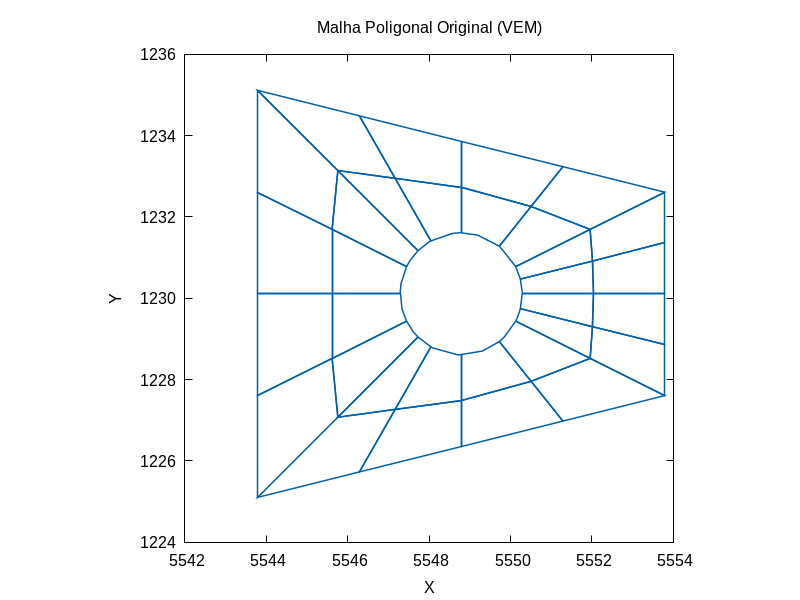
\includegraphics[width=\textwidth]{figuras/Capítulo 5/Placa com furo/malha não deformada 32.png}
            \label{fig:5.3a}
        \end{subfigure}
        \hfill
        \begin{subfigure}[b]{0.45\textwidth}
            \centering
            \caption{malha de 64 elementos}
            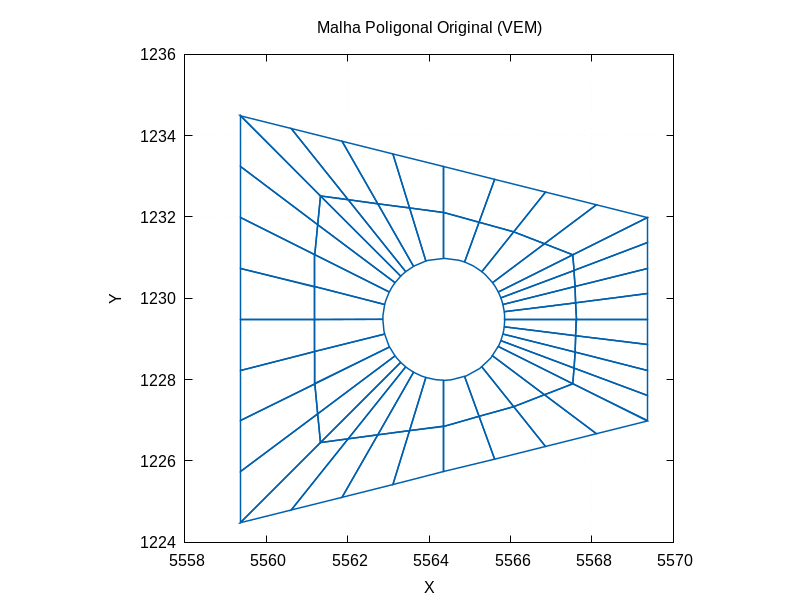
\includegraphics[width=\textwidth]{figuras/Capítulo 5/Placa com furo/mallha não deformada 64.png}
            \label{fig:5.3b}
        \end{subfigure}
        \centerline{{\small \textbf{Fonte:} Elaborado pelo autor (2026).}}
    \end{figure}  

\begin{table}[htbp]
    \centering
    \caption{Erros relativos das frequências para as malhas de 32 e 64 elementos.}
    \label{tab:5.3}
    \small % Reduz o tamanho da fonte para padronização acadêmica
    \begin{tabular}{lccccc}
        \toprule
        \textbf{MODO} & \textbf{PF32N62k1} & \textbf{PF32N82k1} & \textbf{PF32N103k1} & \textbf{PF64N105k1} & \textbf{PF64N114k1} \\
        \midrule
        1  & 12,90\% & 12,90\% & 12,90\% & 19,35\% & 24,73\% \\
        2  & 3,76\%  & 3,76\%  & 2,55\%  & 56,31\% & 49,64\% \\
        3  & 14,36\% & 14,36\% & 14,36\% & 63,02\% & 33,82\% \\
        4  & 24,19\% & 23,85\% & 21,13\% & 58,15\% & 40,46\% \\
        5  & 18,72\% & 18,10\% & 17,79\% & 48,81\% & 38,33\% \\
        6  & 10,71\% & 10,71\% & 7,98\%  & 51,58\% & 50,44\% \\
        7  & 20,71\% & 20,71\% & 19,59\% & 40,87\% & 21,02\% \\
        8  & 9,99\%  & 9,99\%  & 9,19\%  & 29,82\% & 20,17\% \\
        9  & 18,90\% & 17,22\% & 17,40\% & 25,92\% & 21,61\% \\
        10 & 22,88\% & 22,33\% & 19,23\% & 25,43\% & 21,60\% \\
        \bottomrule
    \end{tabular}
    
    \vspace{0.2cm}
    \raggedright
    \textbf{Fonte:} Elaborado pelo autor (2026).
\end{table}

\indent A figura~\ref{fig:5.4} obtidas para cada malha. Percebe-se para a malha de 32 elementos uma melhor aproximação da solução de referência quando comparada à malha de 8 elementos para as primeiras frequências. Contudo, a partir do quarto modo, existe um aumento no valor das frequências em comparação com a malha de 8 elementos. Para a malha de 64 elementos, observa-se uma inversão logo nos primeiros modos, em que a frequência se torna menor que a referência e mantém-se assim para todos os modos subsequentes. Investigando o fenômeno mais a fundo, calcularam-se os erros relativos de cada frequência ilustrados na Figura~\ref{fig:5.4}.

\begin{figure}[H]
    \centering
    \caption{Comparação das frequências obtidas por modo de vibração para a chapa engastada com furo.}
    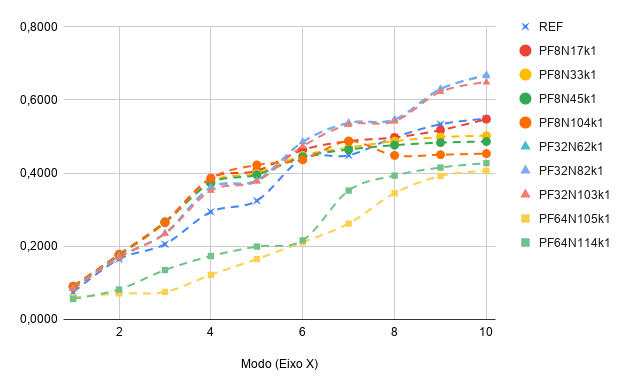
\includegraphics[width=\textwidth]{figuras/Capítulo 5/Placa com furo/Comparação de frequências com modos de vibração - Placa engastada com furo.png}
    \label{fig:5.4}
    \centerline{    {\small \textbf{Fonte:} Elaborado pelo autor (2026).}}

\end{figure}

\indent Da Figura~\ref{fig:5.4}, constata-se que: 

\begin{itemize}
    \item As malhas de 32 elementos apresentam frequências similares às de referência apenas para os primeiros modos de vibração.
    \item A malha com 64 elementos apresenta valores muito inferiores aos de referência, mesmo com o aumento da quantidade de graus de liberdade.
    \item As curvas variam entre si conforme a quantidade de elementos, mas o valor o das frequências nas malhas com a mesma quantidade de elementos apresenta pouca variação entre si.
\end{itemize}

\indent Para compreender o fenômeno que ocorre nas malhas de 64 elementos, analisa-se o condicionamento das matriz de massa e rigidez (Figura~\ref{fig:5.5}):

\begin{figure}[H]
    \centering
    \caption{Condicionamento de $K$ em função das malhas utilizadas.}
    \label{fig:5.5}
    \begin{subfigure}[b]{0.45\textwidth}
        \centering
        \caption{Matriz K}
        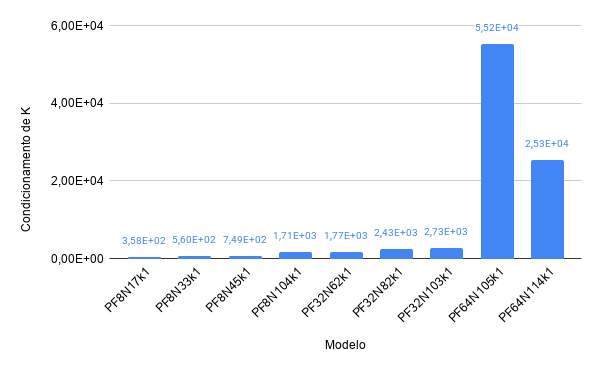
\includegraphics[width=\textwidth]{figuras/Capítulo 5/Placa com furo/Condicionamento de K por malha.png}
        \label{fig:5.5a}
    \end{subfigure}
    \hfill
    \begin{subfigure}[b]{0.45\textwidth}
        \centering
        \caption{Matriz M}
        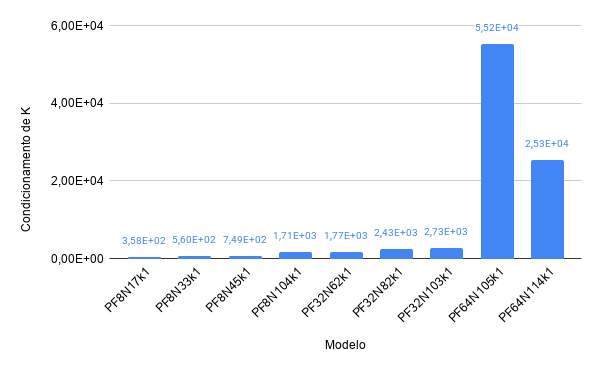
\includegraphics[width=\textwidth]{figuras/Capítulo 5/Placa com furo/Condicionamento de K por malha.png}
        \label{fig:5.5b}
    \end{subfigure}
    

    {\small \textbf{Fonte:} Elaborado pelo autor (2026).}
\end{figure}

\indent Observa-se na Figura~\ref{fig:5.5} que o valor do condicionamento da matriz de rigidez para a primeira malha de 64 elementos assume valores maiores que $6 \times 10^4$. Como destacado por \citet{stabilityanalysisvirtualelementmethod2016a}, polígonos com arestas muito menores que o diâmetro dos elementos comprometem a coercividade da constante de estabilidade, e \citet{illconditioningvirtualelementmethodstabilizationsbases2018} demonstra que polígonos malformados comprometem o condicionamento. O excesso de elementos na malha mais refinada faz com que os elementos que fazem fronteira com o furo possuam arestas muito pequenas, prejudicando a estabilidade do método.\\
\indent Buscando validar os resultados, foram calculados os erros MAPE, NRMSE e MG para cada uma das malhas. Os resultados estão resumidos na Tabela~\ref{tab:5.6} e a curva entre os erros é apresentada na Figura~\ref{fig:5.6}.

\begin{figure}[H]
    \centering
    \caption{Curva de erros para a chapa engastada com furo.}
    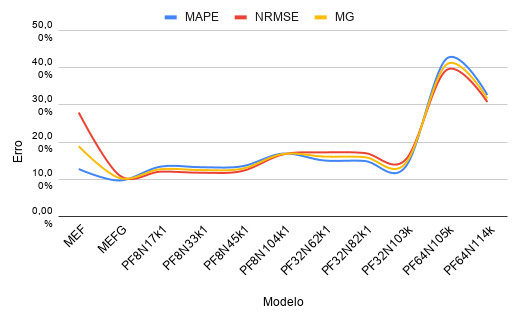
\includegraphics[width=0.9\textwidth]{figuras/Capítulo 5/Placa com furo/Curva de erros - Placa engastada com furo.png}
    \label{fig:5.6}

    \centerline{    {\small \textbf{Fonte:} Elaborado pelo autor (2026).}}
\end{figure}


\begin{table}[htbp]
    \centering
    \caption{Métricas de erro global (MAPE, NRMSE e MG) para cada malha da chapa engastada.}
    \label{tab:5.6}
    \setlength{\tabcolsep}{3pt} % Ajusta o espaçamento entre colunas para caber na página
    \small % Reduz o tamanho da fonte para o padrão acadêmico
    \begin{tabular}{lccccccccc}
        \toprule
        \multirow{2}{*}{\textbf{Média}} & \multicolumn{4}{c}{\textbf{8 elementos}} & \multicolumn{3}{c}{\textbf{32 elementos}} & \multicolumn{2}{c}{\textbf{64 elementos}} \\
        \cmidrule(lr){2-5} \cmidrule(lr){6-8} \cmidrule(lr){9-10}
        & \textbf{(34 gl)} & \textbf{(66 gl)} & \textbf{(90 gl)} & \textbf{(208 gl)} & \textbf{(124 gl)} & \textbf{(164 gl)} & \textbf{(206 gl)} & \textbf{(210 gl)} & \textbf{(228 gl)} \\
        \midrule
        MAPE  & 13,41\% & 13,25\% & 13,50\% & 16,92\% & 15,06\% & 14,93\% & 13,38\% & 42,41\% & 32,67\% \\
        NRMSE & 12,05\% & 11,77\% & 12,22\% & 16,69\% & 17,23\% & 17,06\% & 15,28\% & 39,37\% & 30,78\% \\
        MG    & 12,71\% & 12,48\% & 12,84\% & 16,81\% & 16,11\% & 15,96\% & 14,30\% & 40,86\% & 31,71\% \\
        \bottomrule
    \end{tabular}
    
    \vspace{0.2cm}
    \raggedright
    \textbf{Fonte:} Elaborado pelo autor (2026).
\end{table}

\indent Na curva da figura~\ref{fig:5.6} enquanto os erros do MEV e do MEFG são uniformes, para o MEF existe uma grande diferença entre a MAPE e a NRMSE. Para investigação do fenômeno, construi-se um gráfico (figura~\ref{fig:5.7}) dos erros relativos de cada modo de vibração. A divergência dos erros do MEF é causada principalmente pelas frequências acima do sexto modo de vibração. Nota-se que o MEV apresenta soluções mais acuradas para os modos de vibração mais altos, todavia, os erros relativos percentuais são superiores aos do MEF e do MEFG para os modos iniciais.

\begin{figure}[H]
    \centering
    \caption{Curva de erros relativos por modo de vibração para a chapa com furo}
    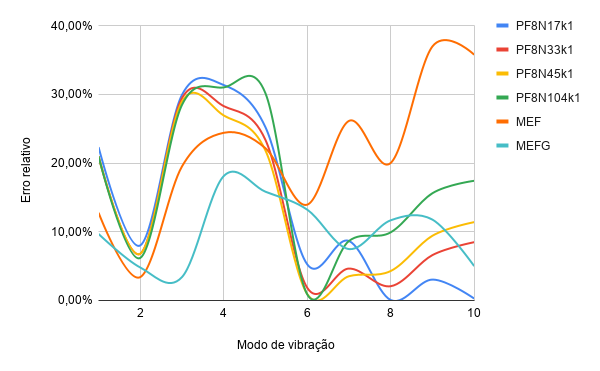
\includegraphics[width=\textwidth]{figuras/Capítulo 5/Placa com furo/Erros relativos.png}
    \label{fig:5.7}

    \centerline{    {\small \textbf{Fonte:} Elaborado pelo autor (2026).}}
\end{figure}

\indent Os dados do ganho de acurácia se encontram na figura~\ref{fig:5.8}. Foi adotada a malha de 8 elementos e 34 graus de liberdade como a malha mais grosseira e a malha de 64 elementos e 228 gl como a mais refinada. Os ganho de discretização da malha de 8 elementos foi pouco expressivo, com queda absoluta de 1,2 pontos percentuais. A malha com maior perda de acurácia foi a malha de 64 elementos e 210 gl alcançando uma queda de 148,15 pontos percentuais.

\begin{figure}[H]
    \centering
    \caption{Coeficiente de acurácia global para as malhas da chapa engastada.}
    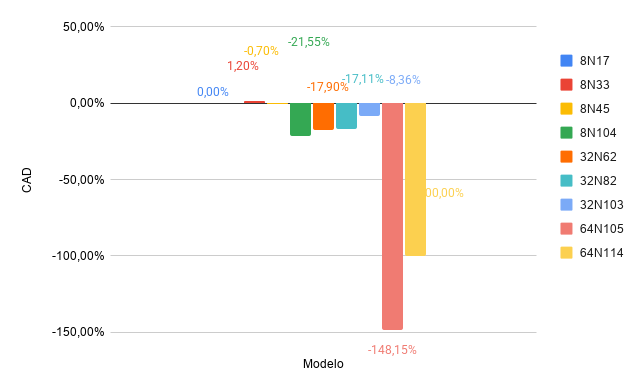
\includegraphics[width=\textwidth]{figuras/Capítulo 5/Placa com furo/CAD - Placa engastada com furo.png}
    \label{fig:5.8}

    \centerline{    {\small \textbf{Fonte:} Elaborado pelo autor (2026).}}
\end{figure}

\indent Analisando os erros, nota-se que a malha com os menores erros é a de 8 elementos a de 32. \citet{basicprinciplesvirtualelementmethods2013a} comentam que o Método dos Elementos Virtuais apresenta a capacidade de lidar com elementos contendo quantidades arbitrárias de nós e formatos complexos, evitando a rigidez artificial imposta pelo particionamento do domínio em elementos padrões.\\
\indent O parâmetro de estabilização utilizado para penalização no termo de estabilidade emprega o traço da matriz de rigidez de consistência como constante multiplicativa. Como explicado por \citet{basicformulationsvirtualelementmethodvemfinitedeformations2017}, essa escolha evita o travamento volumétrico e aumenta a robustez computacional para sólidos submetidos a grandes deformações, fazendo com que o termo de estabilização escale na mesma ordem de grandeza da matriz de consistência.\\
\indent Conforme destacado em \citet{illconditioningvirtualelementmethodstabilizationsbases2018}, o espaço de solução local pode ser particionado em uma componente polinomial e outra puramente virtual:

\begin{equation}
    \begin{aligned}
        V_k (\Omega) = \left\{ v_k \in V_k(\Omega) \mid v_k \in \mathbb{P}_k(\Omega) \right\} \oplus \left\{ v_k \in V_k(\Omega) \mid \Pi_k^\nabla v_k = 0 \right\}\\ = \mathbb{P}_k(\Omega) \oplus \ker(\Pi^\nabla_k) = V_{k,1} \oplus V_{k,2}
    \end{aligned}
\end{equation}

\noindent de tal modo que uma função polinomial seja nula no espaço puramente virtual $V_{k,2}$ e uma função virtual se anule no espaço polinomial $V_{k,1}$. Próximo à região do furo, os campos de deformação apresentam elevados gradientes, fazendo com que a projeção polinomial não capture toda a cinemática local e resultando em uma contribuição significativa da componente puramente virtual (e, consequentemente, da matriz de estabilização).\\
\indent Como notado por \citet{virtualelementmethodstekloveigenvalueproblemallowingsmalledges2020a}, o parâmetro de estabilização pode afetar a aproximação do espectro de autovalores, resultando em um problema discreto excessivamente rígido e poluindo severamente as frequências mais altas, particularmente quando malhas distorcidas são empregadas. Assim, com o aumento da quantidade de elementos na região do furo, há também o aumento do número de matrizes de estabilização locais somadas ao sistema, impondo uma rigidez artificial global à solução que degrada os resultados da malha de 32 elementos.\\
\indent Outro detalhe que pode ser visto analisando os resultados das tabelas~\ref{tab:5.3} e \ref{tab:5.2} é a malha de 8 elementos possuir maiores erros em relação aos primeiros modos de vibração quando comparada à malha de 32 elementos. Isso demonstra que o refino de uma malha de 32 seria o ideal se não fossem os erros acumulados da estabilização. Com essa consideração, trabalhos futuros podem realizar essa mesma análise utilizando a formulação livre de estabilização do MEV e comparar os resultados.\\
\indent O estudo do ganho de precisão relativo do método foi executado para a formulação de elementos finitos clássica apresentada no trabalho de \citet{asymptoticsolutionspredictednaturalfrequenciestwodimensionalelasticsolidvibrationproblemsfiniteelementanalysis1996} -- e não a versão com correção assintótica.\\
\indent Através do cálculo do GPR (tabela~\ref{tab:5.7}) são feitas as seguintes observações:
\begin{itemize}
    \item Quando analisada apenas a MAPE conclui-se que não houve ganho de precisão em relação ao MEF em nenhuma malha;
    \item Os valores da NRMSE e da MG são positivos apenas pela penalização imposta pela NRMSE sobre as frequências dos modos mais altos do MEF. 
    \item Avaliando a MG, apenas as malhas de 64 elementos apresentaram perda de precisão.
    \item A malha de 8 elementos e 208 gl apresentou ganho de discretização menor que a malha de 32 elementos e 124 graus de liberdade. Isso pode ser explicado pelo excesso de graus de liberdade no contorno do furo com a formulação atingindo um ponto de saturação na malha de 90 gl.
\end{itemize}


\begin{table}[htbp]
    \centering
    \caption{Ganho de precisão relativo no problema da chapa engastada com furo.}
    \label{tab:5.7}
    \setlength{\tabcolsep}{3pt} % Ajusta o espaçamento lateral para evitar estouro de margem
    \small % Reduz o tamanho da fonte para o padrão acadêmico
    \begin{tabular}{lccccccccc}
        \toprule
        \multirow{2}{*}{\textbf{Média}} & \multicolumn{4}{c}{\textbf{8 elementos}} & \multicolumn{3}{c}{\textbf{32 elementos}} & \multicolumn{2}{c}{\textbf{64 elementos}} \\
        \cmidrule(lr){2-5} \cmidrule(lr){6-8} \cmidrule(lr){9-10}
        & \textbf{(34 gl)} & \textbf{(66 gl)} & \textbf{(90 gl)} & \textbf{(208 gl)} & \textbf{(124 gl)} & \textbf{(164 gl)} & \textbf{(206 gl)} & \textbf{(210 gl)} & \textbf{(228 gl)} \\
        \midrule
        MAPE  & -5\%   & -3,73\% & -5,71\% & -32,53\% & -17,97\% & -16,94\% & -4,79\%  & -232,10\% & -155,86\% \\
        NRMSE & 57\%   & 57,91\% & 56,28\% & 40,29\%  & 38,35\%  & 38,96\%  & 45,34\%  & -40,83\%  & -10,11\%  \\
        MG    & 33\%   & 33,93\% & 32,01\% & 11,04\%  & 14,72\%  & 15,51\%  & 24,32\%  & -116,27\% & -67,85\%  \\
        \bottomrule
    \end{tabular}
    
    \vspace{0.2cm}
    \raggedright
    \textbf{Fonte:} Elaborado pelo autor (2026).
\end{table}

\indent A perda da precisão na malha de 8 elementos e 208 graus de liberdade é explicada pela quantidade excessiva de arestas utilizadas na modelagem do furo por elementos. A aproximação linear permite apenas a representação do campo de deformações constantes por parte da parcela de consistência, com o restante sendo controlado pela parcela de estabilização. Como destacado por \citet{engineeringperspectivevirtualelementmethoditsinterplaystandardfiniteelementmethod2019a}, a função da projeção é garantir que o trabalho virtual interno gerado pelas funções do MEV seja o mesmo provocado pela base polinomial escolhida. Grandes concentrações de nós em uma mesma vizinhança geométrica-elástica fazem com que a base de monômios perca sua independência numérica, tornando a matriz $\mathcal{D}$ praticamente linearmente dependente. Como a técnica de estabilização aplicada utiliza $\mathcal{D}$ em sua construção, derivam-se erros na parcela de estabilização, impondo uma falsa rigidez ao elemento. \citet{illconditioningvirtualelementmethodstabilizationsbases2018} afirma que as diversas técnicas de estabilização presentes na literatura possuem efeitos semelhantes no condicionamento da matriz de rigidez, diferentemente da escolha dos graus de liberdade internos, que possuem grande impacto.\\
\indent Para o estudo da acurácia entre o MEFG e o MEV, utilizam-se os resultados da formulação clássica de elementos finitos como parâmetro de referência de cálculo. Estudando o CA (Tabela~\ref{tab:5.8}), nota-se que a performace do MEV foi inferior a do MEF e do MEFG avaliando a MAPE. Contudo, para a NRMSE e a MG, o resultado foi superior somente ao do MEF.

\begin{table}[htbp]
    \centering
    \caption{Coeficientes de acurácia (CA) entre MEV e MEFG.}
    \label{tab:5.8}
    \small % Reduz o tamanho da fonte para o padrão acadêmico
    \begin{tabular}{lcccc}
        \toprule
        \textbf{Modelo} & \textbf{PF8N17k1} & \textbf{PF8N33k1} & \textbf{PF8N45k1} & \textbf{PF8N104k1} \\
        \midrule
        MAPE  & -0,21 & -0,15 & -0,24 & -1,34 \\
        NRMSE &  0,94 &  0,96 &  0,93 &  0,67 \\
        MG    &  0,72 &  0,75 &  0,71 &  0,24 \\
        \bottomrule
    \end{tabular}
    
    \vspace{0.2cm}
    \raggedright
    \textbf{Fonte:} Elaborado pelo autor (2026).
\end{table}

\indent Como considerações finais desse problema, ressalta-se que, mesmo em problemas com geometrias complexas, a presença de regiões com descontinuidade afeta a aproximação com o MEV. Algumas soluções são a utilização de métodos de partição da unidade junto ao MEV, a aplicação de formulações livres de estabilização ou a adoção da formulação para elementos com arestas curvas.

\section{Barragem de terra}

\indent O terceiro problema a ser estudado é uma barragem de terra modelada pelo estado plano de deformações, (Figura~\ref{fig:5.11}). O modelo de cálculo é um triângulo isósceles com módulo de elasticidade $E = 5,602 \times 10^8\text{ (N/m}^2\text{)}$, densidade $\rho = 2080\text{ (kg/m}^3\text{)}$ e coeficiente de Poisson $\nu = 0,45$.

\begin{figure}[H]
    \centering
    \caption{Geometria da barragem de terra em estado plano de deformações.}
    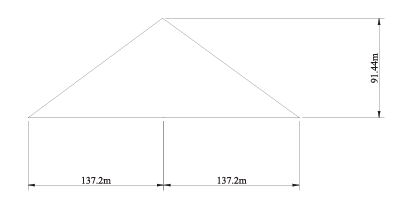
\includegraphics[width=\textwidth]{figuras/Capítulo 5/Barragem/Captura de tela 2026-08-19 082612.png}
    \label{fig:5.11}

    \centerline{    {\small \textbf{Fonte:} Elaborado pelo autor (2026).}}

\end{figure}

\indent O problema de vibrações em barragens de terra foi proposto pela primeira vez por \citet{earthquakestressanalysisearthdams1966}, (Figura~\ref{fig:5.12}), voltado à análise de terremotos em barragens de terra. O mesmo problema foi abordado por \citet{analytictrapezoidalfourierpelementvibratingplaneproblems2004} com a utilização de elementos p-Fourier trapezoidais em problemas de vibração no plano, (Figura~\ref{fig:5.13}), por \citet{refinednonconformingplanequadrilateralelement2000} no desenvolvimento de um elemento quadrilateral plano não conforme refinado, (Figura~\ref{fig:5.14}), e por \citet{cittadin2020enriquecimento} na análise do coeficiente de Friberg junto ao MEFG.

\begin{figure}[H]
    \centering
    \caption{Malha e geometria proposta originalmente.}
    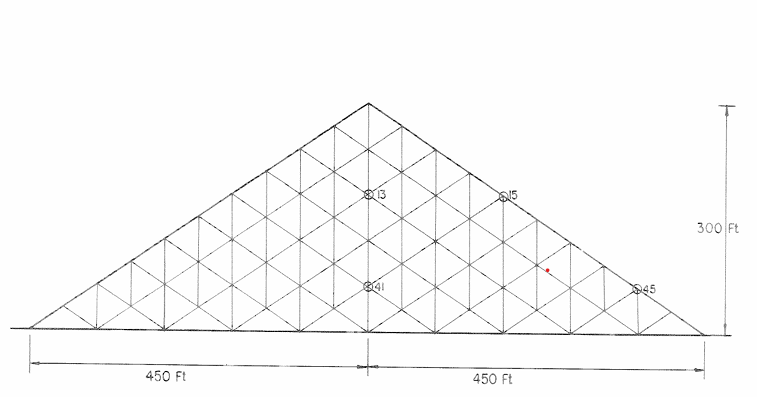
\includegraphics[width=0.8\textwidth]{figuras/Capítulo 5/Barragem/Captura de tela 2026-08-19 083021.png}
    \label{fig:5.12}

    \centerline{    {\small \textbf{Fonte:} \citet{earthquakestressanalysisearthdams1966}.}}

\end{figure}

\begin{figure}[H]
    \centering
    \caption{Discretização por elementos p-Fourier trapezoidais.}
    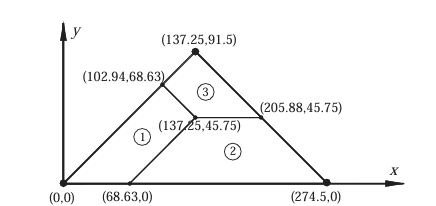
\includegraphics[width=0.9\textwidth]{figuras/Capítulo 5/Barragem/Captura de tela 2026-08-19 082531.png}
    \label{fig:5.13}

    \centerline{    {\small \textbf{Fonte:} \citet{analytictrapezoidalfourierpelementvibratingplaneproblems2004}.}}

\end{figure}

\begin{figure}[H]
    \centering
    \caption{Modelo quadrilateral não conforme.}
    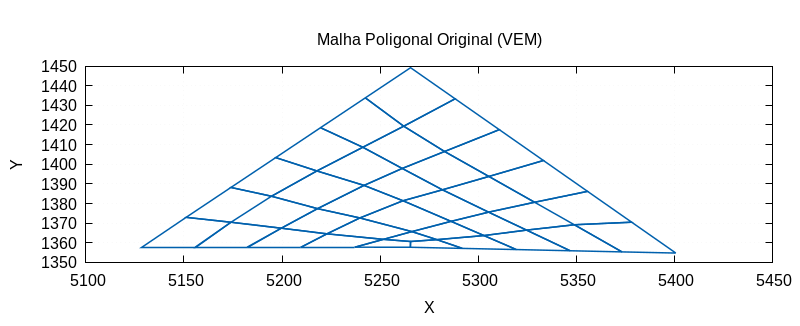
\includegraphics[width=\textwidth]{figuras/Capítulo 5/Barragem/Captura de tela 2026-08-19 082553.png}
    \label{fig:5.14}
    
     {\small \textbf{Fonte:} Elaborado pelo autor (2026).}
\end{figure}

\indent A primeira análise realizada envolve a malha de 3 elementos de \citet{analytictrapezoidalfourierpelementvibratingplaneproblems2004}. A tabela~\ref{tab:5.9a} contém os resultados obtidos pelos autores previamente citados. Para o estudo, foram utilizadas quatro malhas de elementos virtuais, três malhas de 3 elementos (Figura~\ref{fig:5.13}) contendo respectivamente 14 gl, 30 gl e 72 gl e uma malha de 35 elementos e 94 gl (Figura~\ref{fig:5.14}). Essas malhas serão utilizadas como forma de comparação com os resultados obtidos pelos demais autores. Os resultados do MEV se encontram na tabela~\ref{tab:5.9b}

% Certifique-se de ter os pacotes \usepackage{booktabs} e \usepackage{makecell} no preâmbulo.

\begin{table}[htbp]
    \centering
    \caption{Frequências naturais dos autores citados para a barragem de terra (rad/s).}
    \label{tab:5.9a}
    \setlength{\tabcolsep}{4pt} % Ajusta o espaçamento lateral para acomodar os textos dos cabeçalhos
    \small % Reduz o tamanho da fonte para o padrão acadêmico
    \begin{tabular}{lccccc}
        \toprule
        \textbf{Modo} & 
        \makecell{\textbf{\protect\citet{chopra2023dynamics}}\\\textbf{(110 gl)}} & 
        \makecell{\textbf{\protect\citet{analytictrapezoidalfourierpelementvibratingplaneproblems2004}}\\\textbf{(25 gl)}} & 
        \makecell{\textbf{\protect\citet{refinednonconformingplanequadrilateralelement2000}}\\\textbf{(72 gl)}} & 
        \makecell{\textbf{\protect\citet{cittadin2020enriquecimento}}\\\textbf{MEF (25 gl)}} & 
        \makecell{\textbf{\protect\citet{cittadin2020enriquecimento}}\\\textbf{MEFG (182 gl)}} \\
        \midrule
        1 & 7,71  & 7,79  & 7,76  & 7,95  & 7,76  \\
        2 & 12,52 & 12,52 & 12,52 & 17,71 & 12,46 \\
        3 & 14,6  & 14,51 & 14,49 & 23,44 & 14,34 \\
        4 & 19,31 & 18,42 & 18,36 & 30,70 & 18,36 \\
        \bottomrule
    \end{tabular}
    
    \vspace{0.2cm}
    \raggedright
    \textbf{Fonte:} Elaborado pelo autor (2026) a partir de \citet{chopra2023dynamics}, \citet{analytictrapezoidalfourierpelementvibratingplaneproblems2004}, \citet{refinednonconformingplanequadrilateralelement2000} e \citet{cittadin2020enriquecimento}.
\end{table}


\begin{table}[htbp]
    \centering
    \caption{Frequências naturais do MEV para a barragem de terra (rad/s).}
    \label{tab:5.9b}
    \small % Reduz o tamanho da fonte para o padrão acadêmico
    \begin{tabular}{lcccc}
        \toprule
        \multirow{2}{*}{\textbf{Modelo}} & \multicolumn{3}{c}{\textbf{3 elem.}} & \textbf{35 elem.} \\
        \cmidrule(lr){2-4} \cmidrule(lr){5-5}
        & \textbf{(14 gl)} & \textbf{(30 gl)} & \textbf{(72 gl)} & \textbf{(94 gl)} \\
        \midrule
        1 & 8,038  & 7,981  & 7,932  & 7,811  \\
        2 & 20,289 & 19,38  & 14,929 & 14,431 \\
        3 & 21,323 & 21,093 & 15,385 & 18,656 \\
        4 & 26,575 & 23,225 & 15,605 & 24,111 \\
        \bottomrule
    \end{tabular}
    
    \vspace{0.2cm}
    \raggedright
    \textbf{Fonte:} Elaborado pelo autor (2026).
\end{table}

\indent Como comentado por \citet{cittadin2020enriquecimento}, os valores do MEFG apresentam valores menores que as dos demais autores, partindo do pressuposto que a solução converge por valores superiores, isso é um indicativo de que a solução do MEFG é mais precisa que a dos demais autores considerando, principalmente, a maior quantidade de gl envolvidos. \\
\indent Tomando a solução de \citet{cittadin2020enriquecimento} como referência, calculam-se os erros relativos obtidos pelo MEV para os quatro primeiros modos de vibração. A figura~\ref{fig:5.15} apresenta erros relativos para os quatro primeiros modos de vibração junto aos resultados do MEF obtidos por \citet{cittadin2020enriquecimento}. O MEF apresenta uma significativa deterioração a partir do modo com maior erro na terceira frequência igual à 67,21\%. \\
\indent Os erros do MEV tem características distintas a depender da quantidade de elementos e, a quantidade e distribuição dos gl. As malhas BT3N7 e BT3N15 possuem erros elevados e maiores que o MEF para os dois primeiros modos, porem menores no terceiro e quarto. A convergência com o aumento da quantidade de gl pode ser observada nas curvas das malhas de 3 elementos com a queda da amplitude da malha mais grosseira para a menos grosseira. Uma verificação de interesse é o comportamento das curvas BT3N36 e BT35N48, onde a primeira possui maiores erros nas frequências iniciais e menores nas maiores frequências ao mesmo tempo que a segunda possui comportamento completamente oposto.

\begin{figure}[H]
    \centering
    \caption{Erros relativos para cada modo de vibração.}
    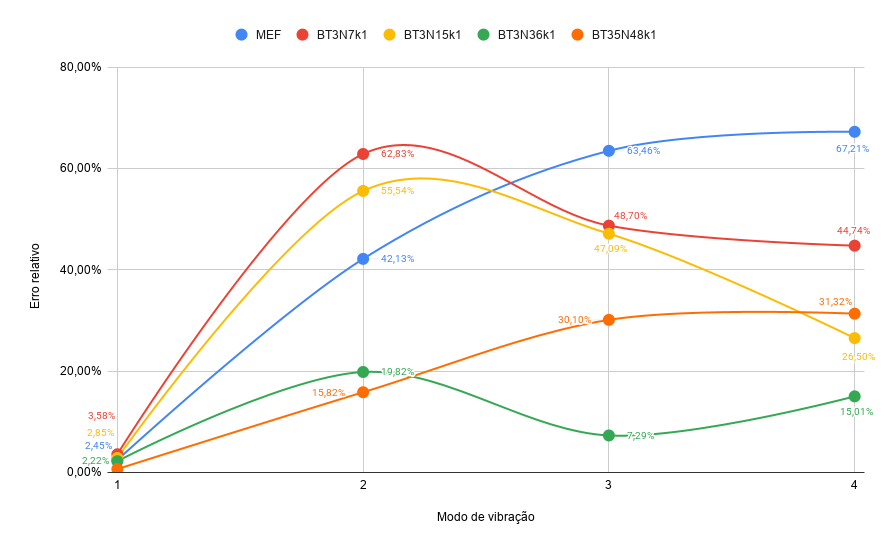
\includegraphics[width=\textwidth]{figuras/Capítulo 5/Barragem/Erro relativo k1.png}
    \label{fig:5.15}

    \centerline{ {\small \textbf{Fonte:} Elaborado pelo autor (2026).}}
\end{figure}

\indent Para uma análise global do desempenho, calculam-se os valores da MAPE, NRMSE e da MG, apresentados na tabela~\ref{tab:5.10b}. Verifica-se que a malha de 72 gl obteve resultados melhores que a malha de 94 gl. \citet{gain2015topology} explica que elementos politópicos com muitos gl atuam como macro-elementos enriquecidos, fornecendo flexibilidade cinemática superior e evitando o travamento numérico. Portanto, poucos elementos altamente enriquecidos são capazes de aproximar a solução melhor que diversos elementos simples.

\begin{table}[htbp]
    \centering
    \caption{Avaliações globais dos erros dos modelos.}
    \label{tab:5.10b}
    \small % Reduz o tamanho da fonte para o padrão acadêmico
    \begin{tabular}{lccccc}
        \toprule
        \multirow{2}{*}{\textbf{Modelo}} & \textbf{MEF} & \multicolumn{3}{c}{\textbf{8 elem.}} & \textbf{35 elem.} \\
        \cmidrule(lr){3-5} \cmidrule(lr){6-6}
        & \textbf{(14 gl)} & \textbf{(14 gl)} & \textbf{(30 gl)} & \textbf{(72 gl)} & \textbf{(94 gl)} \\
        \midrule
        MAPE  & 43,82\% & 39,96\% & 32,99\% & 11,08\% & 19,47\% \\
        NRMSE & 58,86\% & 48,40\% & 39,32\% & 13,98\% & 27,08\% \\
        MG    & 50,79\% & 43,98\% & 36,02\% & 12,44\% & 22,96\% \\
        \bottomrule
    \end{tabular}
    
    \vspace{0.2cm}
    \raggedright
    \textbf{Fonte:} Elaborado pelo autor (2026).
\end{table}


\indent Mesmo com os resultados da malha de 3 elementos e 14 gl obtendo uma resposta melhor que a do MEF com 14 gl, buscou-se obter menores erros nos resultados. Como detalhado por \citet{basicprinciplesvirtualelementmethods2013a}, a acurácia é ditada pelo grau de interpolação $k$ da projeção polinomial, levando a uma taxa de convergência $\mathcal{O}(h^{k+1})$ ótima na norma $L^2$. O aumento do número de arestas não melhora essa taxa teórica se o espaço polinomial se mantiver fixo. Portanto, existe um teto que pode ser assumido pelo termo de consistência e estabilização. \citet{virtualelementmethodwheelrailcontactproblems2021} complementa que grandes espaços de funções virtuais permitem a captura de oscilações, e sua projeção polinomial em espaços polinomiais menores efetivamente os amortece. Assim é proposto o refino-p para os mesmo conjunto de malhas utilizadas. As frequências para o caso $k=2$ estão listadas na tabela~\ref{tab:5.11}

\begin{table}[htbp]
    \centering
    \caption{Frequências obtidas com o refino de malha e ordem polinomial $k=2$.}
    \label{tab:5.11}
    \small % Reduz o tamanho da fonte para o padrão acadêmico
    \begin{tabular}{lcccc}
        \toprule
        \multirow{2}{*}{\textbf{Modelo}} & \multicolumn{3}{c}{\textbf{3 elem.}} & \textbf{35 elem.} \\
        \cmidrule(lr){2-4} \cmidrule(lr){5-5}
        & \textbf{(32 gl)} & \textbf{(64 gl)} & \textbf{(188 gl)} & \textbf{(256 gl)} \\
        \midrule
        1 & 0,000 & 2,521 & 11,074 & 7,726  \\
        2 & 0,000 & 3,410 & 11,191 & 12,879 \\
        3 & 0,000 & 7,069 & 14,141 & 15,519 \\
        4 & 4,304 & 7,699 & 18,020 & 19,189 \\
        \bottomrule
    \end{tabular}
    
    \vspace{0.2cm}
    \raggedright
    \textbf{Fonte:} Elaborado pelo autor (2026).
\end{table}

\indent Similar ao que foi feito para o caso $k=1$, a figura~\ref{fig:5.16} apresenta o comparativo dos erros do MEV com os do MEF. A primeira coisa a ser percebida é as malhas BT3N7k2 e BT3N15k2 apresentarem modos artificiais, com BT3N7k2 apresentando as três primeiras frequências nulas. A malha BT3N36k2 diferente das outras malhas de 3 elementos obteve bons resultados em todas as frequências com exceção da terceira que possui erro de 8,0\%, mas ainda menor que sua contraparte $k=1$.

\begin{figure}[H]
    \centering
    \caption{Erros relativos para cada modo de vibração.}
    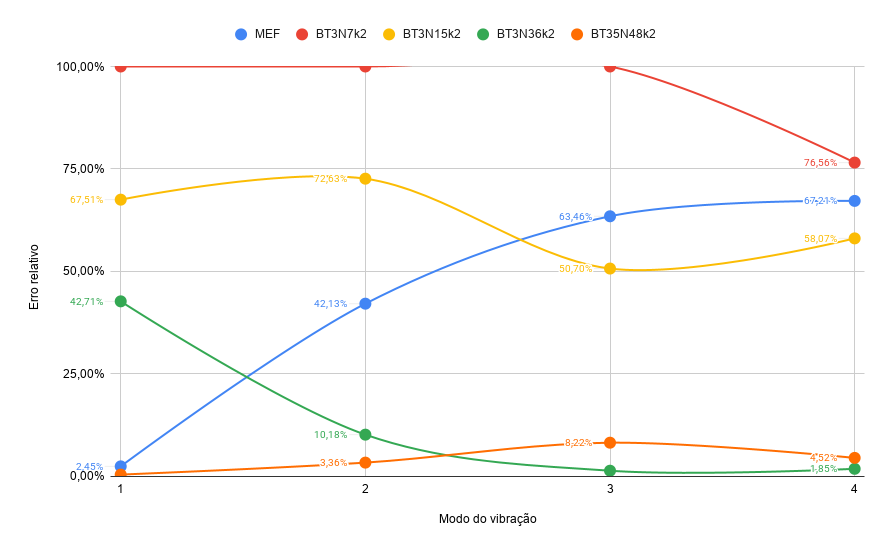
\includegraphics[width=.95\textwidth]{figuras/Capítulo 5/Barragem/Erro relativo k2.png}
    \label{fig:5.16}

    \centerline{ {\small \textbf{Fonte:} Elaborado pelo autor (2026).}}
\end{figure}

\indent Observando os resultados, percebe-se que as malhas de 35 elementos obtiveram resultados muito próximos da solução de referência, com destaque para a malha de segunda ordem com erro máximo de 0,44\%. Porém, os piores resultados foram os das malhas de 3 elementos de segunda ordem, com a malha BT3N7k2 obtendo 94,14\% de erro.\\
\indent Analisando as frequências da malha BT3N7k2, os três primeiros modos foram nulos, o que é um sintoma de modos espúrios de energia. \citet{arbitraryorder2dvirtualelementspolygonalmeshespartelasticproblem2017a} afirma que a função da matriz de estabilização é manter a positividade da forma energética local, e, pela propriedade de estabilidade, a energia elástica computada internamente é equivalente à verdadeira, evitando modos espúrios. Como explicado anteriormente, a norma da forma bilinear é limitada por duas constantes: a constante inferior garante a coercividade e, portanto, a unicidade da solução, enquanto a constante superior garante a continuidade.\\
\indent \citet{virtualelementmethodgeneralsecondorderellipticproblemspolygonalmeshes2016} sustenta que o termo de estabilidade deve ser definido positivo\footnote{O termo de estabilidade é definido positivo quando obtiver um valor positivo ao aplicar a ele uma função $v \in \ker(\Pi_k^\nabla)$ ao mesmo tempo que deve ser nulo para os movimentos de corpo rigido.} no núcleo do projetor $\Pi^\nabla$, garantindo que os únicos modos de energia nula da matriz de rigidez local sejam os movimentos de corpo rígido. A má calibração da matriz de estabilização faz com que o limite inferior tenda a zero, o que implica a perda da capacidade de imposição de resistência elástica às deformações virtuais pertencentes ao $\ker(\Pi_k^\nabla)$ por parte da estabilização, fazendo com que o modelo perca a garantia de unicidade da solução. A malha BT3N7k2 ter seus três primeiros modos nulos é, portanto, um indicador de que a matriz de estabilização perdeu a coercividade.\\
\indent Como notado por \citet{illconditioningvirtualelementmethodstabilizationsbases2018}, a dimensão das componentes é dada por:

\begin{equation}
    \begin{aligned}
        \dim(V_{k,1}(\Omega)) = \dim(\mathbb{P}_{k}(\Omega)) = \frac{(k+1)(k+2)}{2} \\
        \dim(V_{k,2}(\Omega)) = \dim(V_{k}(\Omega)) - \dim(V_{k,1}(\Omega)) = (n_v - 2) k - 1. 
    \end{aligned}
\end{equation}


\indent Assim, nota-se que, com o aumento do grau polinomial, ocorre também um aumento do espaço de solução local. \citet{illconditioningvirtualelementmethodstabilizationsbases2018} também destaca que as constantes $a_*$ e $a^*$ têm uma forte dependência com o grau de interpolação, propriedade demonstrada por \citet{exponentialconvergencehpvirtualelementmethodpresencecornersingularities2018}. Essa propriedade implica que a estabilização é bastante sensível a formulações de alta ordem.\\
\indent \citet{engineeringperspectivevirtualelementmethoditsinterplaystandardfiniteelementmethod2019a} explica que a estabilização deve apenas escalar de maneira apropriada, por exemplo, ter a mesma ordem de magnitude que o termo de consistência independentemente da malha. Malhas grosseiras apresentam elementos com grandes proporções; uma má calibragem do parâmetro de estabilização ou um subdimensionamento em relação à escala física do elemento faz com que a estabilização se torne insignificante em relação ao termo de consistência, o que faz com que o limite inferior tenda a zero. \citet{quantitativestudystabilizationparametervirtualelementmethod2024} afirmam que, conforme a malha é refinada, a solução virtual se torna insensível ao parâmetro de estabilização porque os modos artificiais passam a possuir menores componentes na solução exata e, mesmo que sua energia não seja exata, seu impacto na solução não é severo.\\
\indent A falha das malhas grossas de segunda ordem pode ser explicada como a soma dos fenômenos de subdimensionamento do parâmetro de estabilização em relação à parcela de consistência somada à sensibilidade das constantes limites de estabilização ao aumento do grau de interpolação, de modo que a matriz de estabilização perde a coercividade e modos artificiais aparecem.\\
\indent Um efeito interessante a ser notado é o aumento do número de condicionamento durante a transição de um problema de primeira para segunda ordem, (Figura~\ref{fig:5.17}). \citet{virtualelementmethodtopologyoptimizationpolygonalmeshesnumericalstudy2016} aponta que formulações de elementos virtuais de alta ordem e insuficiência de estabilização em malhas grosseiras levam a elevados números de condicionamentos das matrizes do sistema e ao aparecimento de modos cinemáticos irrestritos.

\begin{figure}[H]
    \centering
    \caption{Condicionamento das matrizes de massa e rigidez do problema da barragem de terra.}
    \label{fig:5.17}
    \begin{subfigure}[b]{0.4\textwidth}
        \centering
        \caption{Condicionamento de $K$.}
        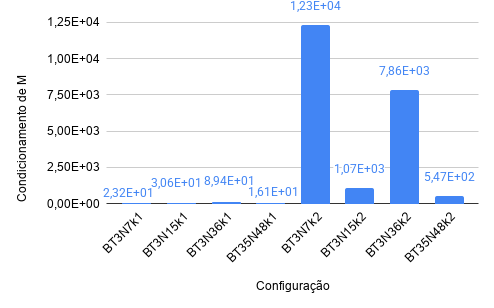
\includegraphics[width=1.2\textwidth]{figuras/Capítulo 5/Barragem/Condicionamento de K - Barragem de terra.png}
        \label{fig:5.17a}
    \end{subfigure}
    \hfill
    \begin{subfigure}[b]{0.4\textwidth}
        \centering
        \caption{Condicionamento de $M$.}
        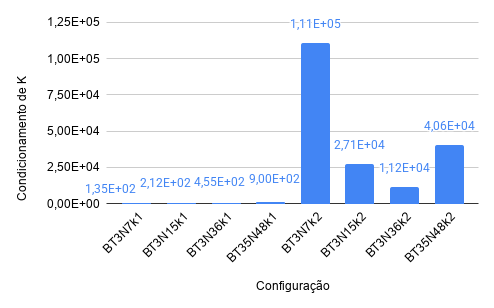
\includegraphics[width=1.2\textwidth]{figuras/Capítulo 5/Barragem/Condicionamento de M - Barragem de terra.png}
        \label{fig:5.17b}
    \end{subfigure}
    
    \centerline{{\small \textbf{Fonte:} Elaborado pelo autor (2026).}}
\end{figure}

\indent Para a análise global dos erros recorre-se novamente a MAPE, NRMSE e a MG descritas na tabela~\ref{tab:5.16b}. Para o caso $k=2$ nota-se um aumento do erro global de solução para as malhas de 3 elementos em relação ao caso $k=1$. Diferente do caso $k=1$, os resultados da malha de 35 elementos obteve melhores resultados que a malha de 3 elementos mais refinada.

\begin{table}[htbp]
    \centering
    \caption{Avaliações globais dos erros dos modelos para $k=2$.}
    \label{tab:5.16b}
    \small % Reduz o tamanho da fonte para o padrão acadêmico
    \begin{tabular}{lcccc}
        \toprule
        \multirow{2}{*}{\textbf{Modelo}} & \multicolumn{3}{c}{\textbf{8 elem.}} & \textbf{35 elem.} \\
        \cmidrule(lr){2-4} \cmidrule(lr){5-5}
        & \textbf{(32 gl)} & \textbf{(64 gl)} & \textbf{(188 gl)} & \textbf{(256 gl)} \\
        \midrule
        MAPE  & 94,14\% & 62,23\% & 14,03\% & 4,13\% \\
        NRMSE & 90,33\% & 60,32\% & 12,97\% & 5,45\% \\
        MG    & 92,22\% & 61,27\% & 13,49\% & 4,75\% \\
        \bottomrule
    \end{tabular}
    
    \vspace{0.2cm}
    \raggedright
    \textbf{Fonte:} Elaborado pelo autor (2026).
\end{table}

\indent Utilizando as médias geométricas dos erros descritas nas tabelas~\ref{tab:5.10b} e \ref{tab:5.16b} calculam-se os valores dos coeficientes de acurácia de discretização apresentados na figura~\ref{fig:5.19}. Para o caso $k=1$ o aumento da precisão estão atrelados ao aumento do número de graus de liberdade com exceção da malha de 35 elementos que apesar de possuir mais gl apresenta resultados em até 1,5 vezes menores que a malha de 3 elementos e 72 gl. Para o caso $k=2$ observa-se um ganho de acurácia proporcional à quantidade de gl do modelo, com a exceção da malha BT3N7k2 que possui as frequências dos três primeiros modos de vibração nulos.

\begin{figure}[H]
    \centering
    \caption{Coeficiente de acurácia de discretização para as malhas da barragem de terra.}
    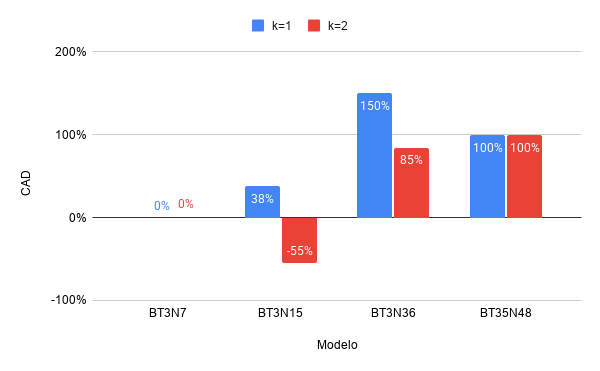
\includegraphics[width=0.8\textwidth]{figuras/Capítulo 5/Barragem/CAD médio.png}
    \label{fig:5.19}

    \centerline{{\small \textbf{Fonte:} Elaborado pelo autor (2026).}}
\end{figure}

\indent Para o cálculo do ganho de precisão, serão descartadas as malhas BT3N7 e BT3N15 para ambos os casos $k=1$ e $k=2$. O ganho de precisão das malhas está sumarizado na Tabela~\ref{tab:5.15}. 

\begin{table}[htbp]
    \centering
    \caption{Ganho de precisão relativo do MEV em relação ao MEF.}
    \label{tab:5.15}
    \small % Reduz o tamanho da fonte para o padrão acadêmico
    \begin{tabular}{lcccc}
        \toprule
        \textbf{Modelo} & \textbf{BT3N36k1} & \textbf{BT35N48k1} & \textbf{BT3N36k1} & \textbf{BT35N48k2} \\
        \midrule
        MAPE  & 74,71\% & 55,56\% & 67,98\% & 90,57\% \\
        NRMSE & 76,26\% & 54,00\% & 77,97\% & 90,74\% \\
        MG    & 75,50\% & 54,79\% & 73,44\% & 90,65\% \\
        \bottomrule
    \end{tabular}
    
    \vspace{0.2cm}
    \raggedright
    \textbf{Fonte:} Elaborado pelo autor (2026).
\end{table}


\section{Parede estrutural}

\indent O quarto problema abordado consiste em uma parede estrutural no estado plano de tensões (Figura~\ref{fig:5.23}). A parede possui módulo de elasticidade $E = 1{,}0 \times 10^{4}\,\text{N/m}^{2}$, coeficiente de Poisson $\nu = 0{,}2$, massa específica $\rho = 1\,\text{kg/m}^{3}$ e espessura $d = 1\,\text{m}$. 
O problema foi proposto em \citet{nguyenthanh2010alternative} como ``benchmark'' para uma formulação alternativa do Método dos Elementos Finitos $\alpha$ (A~$\alpha$~FEM). Os autores comparam a solução com elementos finitos triangulares padrão, uma solução via software ABAQUS, o Método dos Elementos de Contorno e o método sem malha de Petrov-Galerkin local. 

\begin{figure}[H]
    \centering
    \caption{Geometria e modelo da parede estrutural.}
    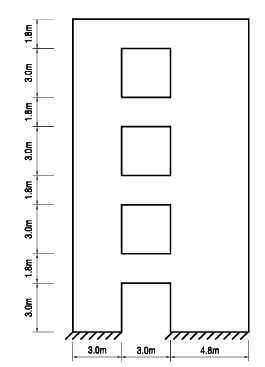
\includegraphics[width=0.5\textwidth]{figuras/Capítulo 5/Parede estrutural/sheer wall.png}
    \label{fig:5.23}

    \centerline{    {\small \textbf{Fonte:} Elaborado pelo autor (2026).}}
\end{figure}

\indent O mesmo problema foi abordado por \citet{custodio2022metodo} com a utilização do MEFG enriquecido com funções trigonométricas. O autor apresenta a comparação entre um elemento enriquecido completo e um elemento enriquecido apenas com funções do tipo bolha. O autor utiliza como referência o A~$\alpha$~FEM de \citet{nguyenthanh2010alternative} e duas famílias de elementos triangulares do MEF, a primeira com aproximação linear e a segunda quadrática.\\
\indent Para a investigação do problema, são utilizados apenas elementos triangulares em malhas uniformes. Inicialmente, elaboram-se quatro diferentes malhas com todos os elementos triangulares: PE40N48k1, PE112N66k1, PE360N262k1 e PE1000N588k1, (Figura~\ref{fig:5.24}). Nota-se que, diferentemente dos problemas anteriores, o aumento da quantidade de elementos é muito maior do que a quantidade de nós ao refinar a malha. \\

\begin{figure}[H]
    \centering
    \caption{Discretizações triangulares para o problema da parede estrutural.}
    \label{fig:5.24}
    \begin{subfigure}[htpb]{0.45\textwidth}
        \centering
        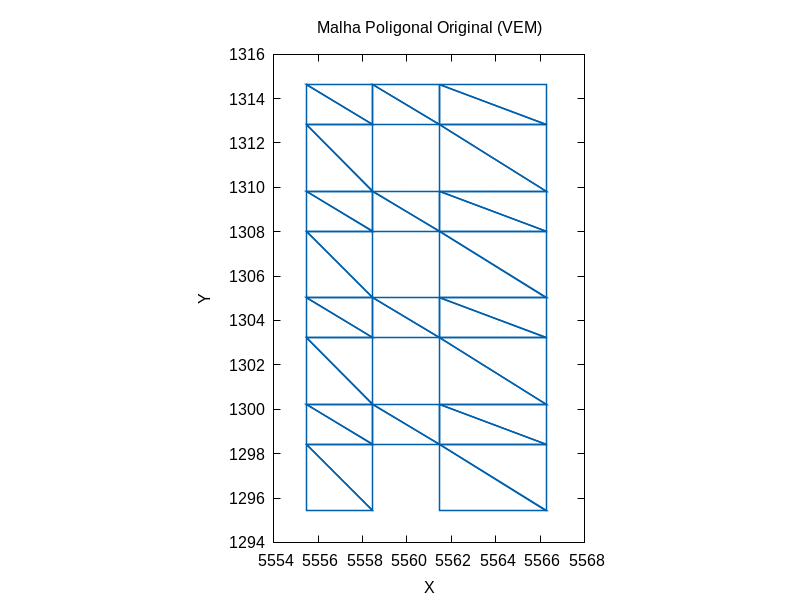
\includegraphics[width=0.8\textwidth]{figuras/Capítulo 5/Parede estrutural/mesh_original 40.png}
        \label{fig:5.24a}
    \end{subfigure}
    \begin{subfigure}[htpb]{0.45\textwidth}
        \centering
        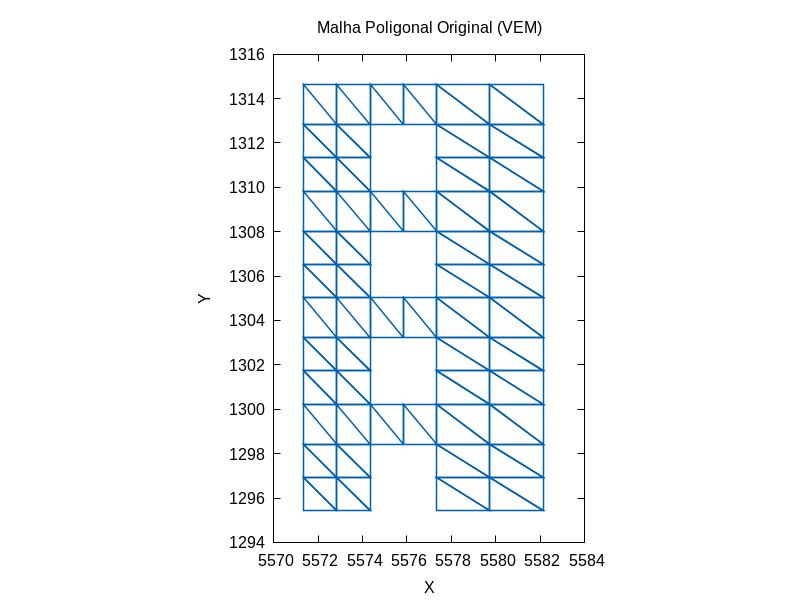
\includegraphics[width=0.8\textwidth]{figuras/Capítulo 5/Parede estrutural/mesh_original 112.png}
        \label{fig:5.24b}
    \end{subfigure}
    \vspace{2mm}
    \begin{subfigure}[htpbb]{0.45\textwidth}
        \centering
        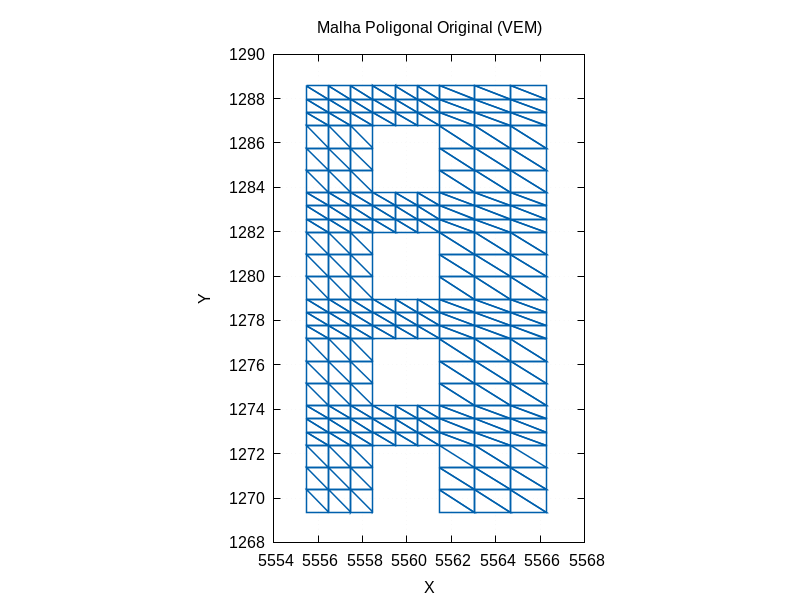
\includegraphics[width=0.8\textwidth]{figuras/Capítulo 5/Parede estrutural/mesh_original 360.png}
        \label{fig:5.24c}
    \end{subfigure}
    \begin{subfigure}[htpb]{0.45\textwidth}
        \centering
        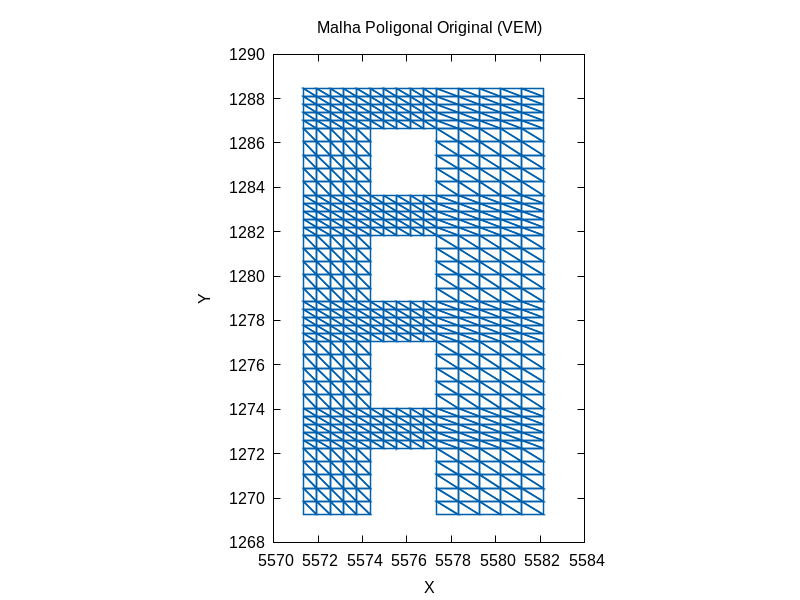
\includegraphics[width=0.8\textwidth]{figuras/Capítulo 5/Parede estrutural/mesh_original 1000.png}
        \label{fig:5.24d}
    \end{subfigure}
    \centerline{    {\small \textbf{Fonte:} Elaborado pelo autor (2026).}}

\end{figure}  


\indent Para o cálculo do erros relativos, como não há solução analítica, utiliza-se o A~$\alpha$~FEM de \citet{nguyenthanh2010alternative}. Os erros estão plotados na Figura~\ref{fig:5.17}. Observam-se erros de até 250\% em relação à solução de referência e mesmo com o aumento da quantidade de elementos os erros sofrem pouca ou nenhuma alteração, sinal de que está ocorrendo travamento numérico.

\begin{figure}[H]
    \centering
    \caption{Erros relativos dos modos de vibração da parede estrutural}
    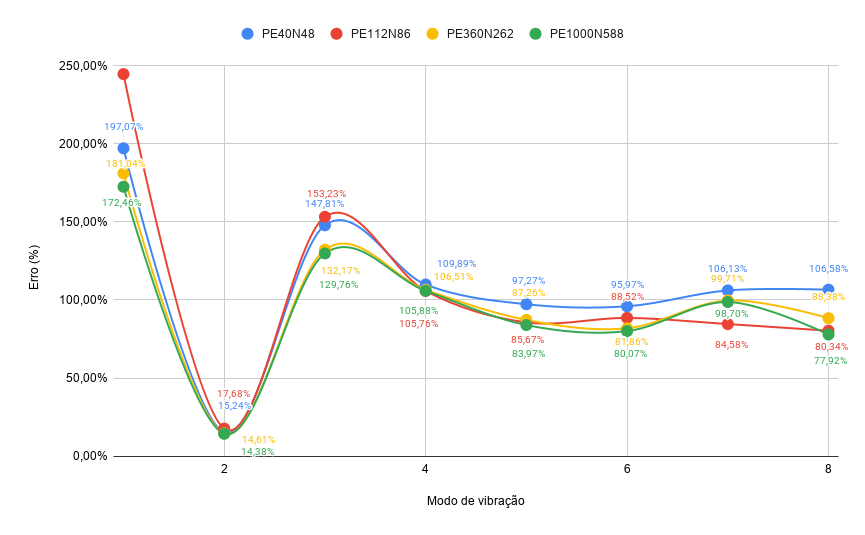
\includegraphics[width=0.9\textwidth]{figuras/Capítulo 5/Parede estrutural/Erros relativos k1.png}
    \label{fig:5.17}

    \centerline{{\small \textbf{Fonte:} Elaborado pelo autor (2026).}}
\end{figure}


\indent  Para verificar as hipóteses analisam-se os números de condicionamento das matrizes de massa e rigidez. Comparando os números de condicionamentos da matriz de rigidez, (Figura~\ref{fig:5.26}), percebe-se que há um aumento expressivo do número de condicionamento

\begin{figure}[H]
    \centering
    \caption{Condicionamento das matrizes de massa e rigidez para as malhas triangulares de primeira ordem.}
    \label{fig:5.26}
    \begin{subfigure}[b]{0.4\textwidth}
        \centering
        \caption{}
        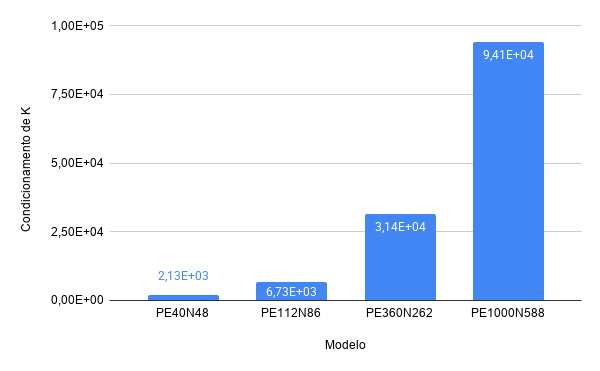
\includegraphics[width=\textwidth]{figuras/Capítulo 5/Parede estrutural/Condicionamento de K para as malhas triangulares.png}
    \end{subfigure}
    \hfill
    \begin{subfigure}[b]{0.4\textwidth}
        \centering
        \caption{}
        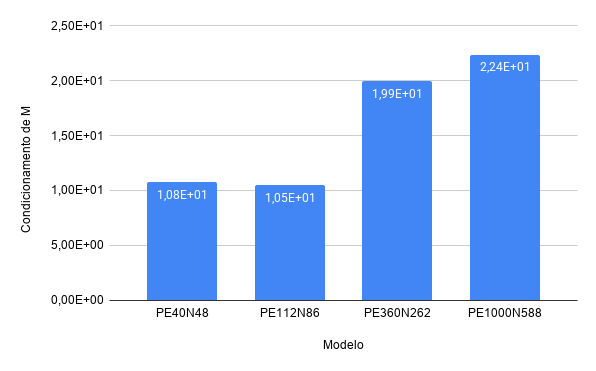
\includegraphics[width=\textwidth]{figuras/Capítulo 5/Parede estrutural/Condicionamento de M para as malhas triangulares.png}
    \end{subfigure}


    \centerline{    {\small \textbf{Fonte:} Elaborado pelo autor (2026).}}
\end{figure}

\indent Para investigar a possibilidade de travamento numérico, utiliza-se o índice $$r_i^{(N)} = \frac{W_{N,i}}{W_{N,i} + W_{S,i}}$$ e $$r_i^{(S)} = \frac{W_{S,i}}{W_{N,i} + W_{S,i}},$$ onde $W_{S,i}$ é a energia de deformação de cisalhamento e $W_{N,i}$ a energia de deformação normal avaliadas por modo de vibração.\\
\indent A figura~\ref{fig:5.18} apresentam mapas com os valores de $r_1^{(N)}$ e $r_1^{(S)}$ para a malha de 1000 elementos. No mapa de deformação volumétrica existem alguns picos de cisalhamento nos montantes, o que é um comportamento normal e esperado, e baixas tensões no interior do modelo, indicativo que não há engessamento volumétrico. Para a energia de deformação de cisalhamento, existem picos de tensões em regiões que deveriam ser dominadas por flexão.

\begin{figure}[H]
    \centering
    \caption{Mapas de energia de deformação por elemento do primeiro modo de vibração para as malhas mais grosseira e mais refinada.}
    \label{fig:5.18}
    \begin{subfigure}[b]{0.4\textwidth}
        \centering
        \caption{Energia de deformação volumétrica}
        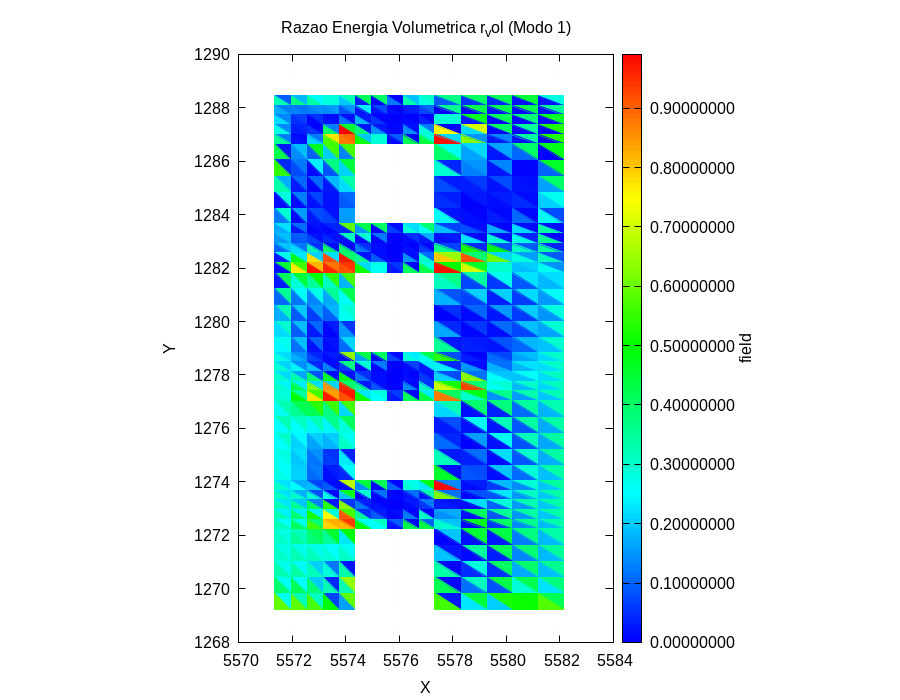
\includegraphics[width=\textwidth]{figuras/Capítulo 5/Parede estrutural/locking_rvol_mode1 PE1000N588.png}
    \end{subfigure}
    \hspace{5mm}
    \begin{subfigure}[b]{0.4\textwidth}
        \centering
        \caption{Energia de deformação de cisalhamento}
        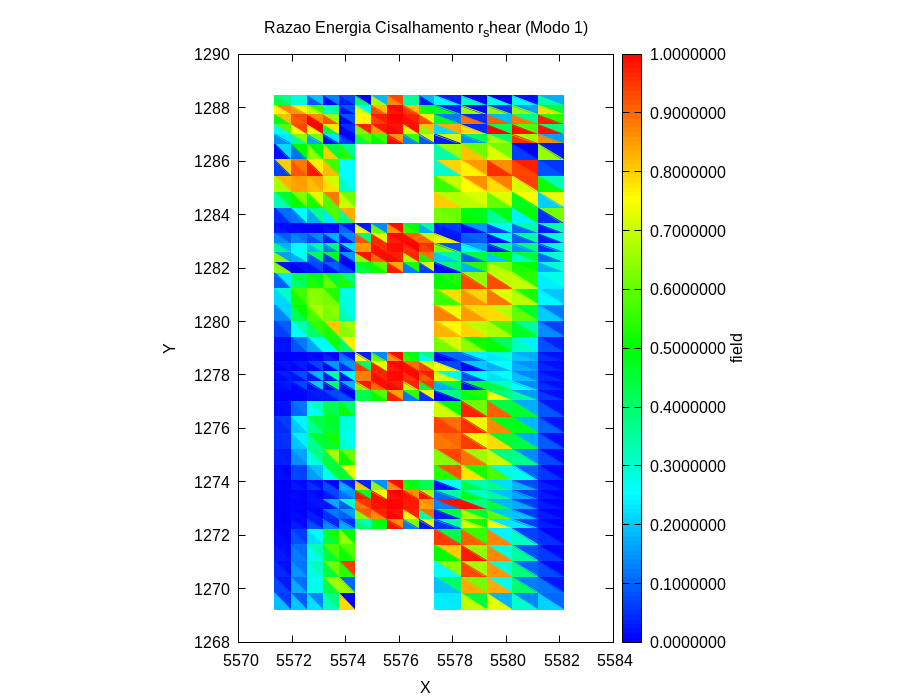
\includegraphics[width=\textwidth]{figuras/Capítulo 5/Parede estrutural/locking_rshear_mode1 PE1000N588.png}
    \end{subfigure}


    \centerline{    {\small \textbf{Fonte:} Elaborado pelo autor (2026).}}
\end{figure}


\indent \citet{hughes1987finite} diz que a norma de energia do erro é severamente poluída pelos termos de cisalhamento quando polinômios de baixa ordem são aplicados a estruturas delgadas, resultando em um fenômeno de travamento no espectro de autovalores. após os teste das hipóteses confirma-se que o erro estava sendo causado por conta da baixa aproximação polinomial. Assim, criaram-se as malhas PE40N48k2, PE112N66k2, PE360N262k2 e PE1000N588k2. Essas malhas apresentam a mesma quantidade de elementos que suas contrapartes de ordem 1, mas com a adição dos nós de aresta e do momento interno característicos de formulações de elementos virtuais de segunda ordem.\\
\indent Assim como feito para o caso $k=1$, a figura~\ref{fig:5.19} traz a comparação dos erros relativos por modo de vibração para quando $k=2$. Comparando as figuras~\ref{fig:5.17} e \ref{fig:5.19} É percebida uma grande queda dos erros assim como a convergência das frequenciais com o aumento de elementos da malha, o que não ocorria para $k=1$.

\begin{figure}[H]
    \centering
    \caption{Erros relativos dos modos de vibração da parede estrutural com $k=2$ e a massa estabilizada pelo diâmetro do elemento}
    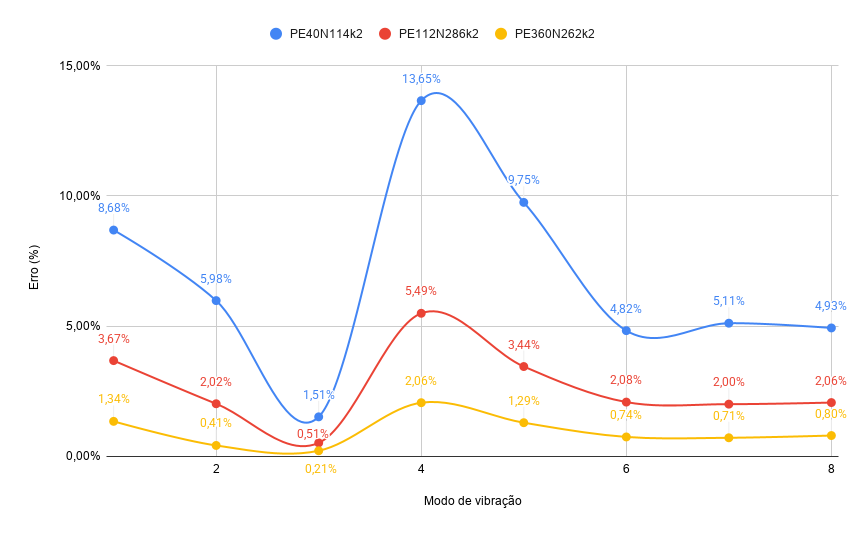
\includegraphics[width=0.8\textwidth]{figuras/Capítulo 5/Parede estrutural/Erros relativos k2.png}
    \label{fig:5.19}

    \centerline{{\small \textbf{Fonte:} Elaborado pelo autor (2026).}}
\end{figure}


\indent Mesmo com os bons resultados obtidos, buscou-se fazer uma investigação do parâmetro de estabilização de massa com a utilização do diâmetro, levando em consideração que $h_E^2$ corresponde ao dobro de $|\Omega_v|^2$ em triângulos. A tabela~\ref{tab:5.20} apresenta as médias globais para diferentes parâmetros de estabilização de massa. 

\begin{table}[htbp]
    \centering
    \caption{Médias globais dos erros do problema da parede estrutural com diferentes parâmetros de estabilização de massa.}
    \label{tab:5.20}
    \setlength{\tabcolsep}{3pt} % Ajusta o espaçamento lateral para evitar estouro de margem
    \small % Reduz o tamanho da fonte para o padrão acadêmico
    \begin{tabular}{lcccccc}
        \toprule
        \multirow{2}{*}{\textbf{Modelo}} & \multicolumn{3}{c}{\textbf{Área}} & \multicolumn{3}{c}{\textbf{Diâmetro}} \\
        \cmidrule(lr){2-4} \cmidrule(lr){5-7}
        & \textbf{PE40N114k2} & \textbf{PE112N286k2} & \textbf{PE360N262k2} & \textbf{PE40N114k2} & \textbf{PE112N286k2} & \textbf{PE360N578k2} \\
        \midrule
        MAPE  & 6,80\% & 2,66\% & 0,94\% & 6,66\% & 2,64\% & 0,94\% \\
        NRMSE & 6,83\% & 2,68\% & 0,99\% & 6,64\% & 2,65\% & 0,99\% \\
        MG    & 6,82\% & 2,67\% & 0,97\% & 6,65\% & 2,64\% & 0,96\% \\
        \bottomrule
    \end{tabular}
    
    \vspace{0.2cm}
    \raggedright
    \textbf{Fonte:} Elaborado pelo autor (2026).
\end{table}

\indent Ao avaliar os resultados globais é possível perceber que a estabilização da matriz de massa é mais proeminente nas malhas mais grosseiras, ao passo que nas malhas mais refinadas a estabilização da massa pouco afeta o resultado geral. Isso está consoante às conclusões de \citet{boffi2026virtual}, que provam que em problemas de autovalores auto adjuntos elípticos a parcela de estabilização da massa pode ser desconsiderada para formulações padrões de baixa e alta ordem.\\
\indent Para um estudo mais aprofundado, plota-se os valores dos erros relativos por modo de vibração (Figura~\ref{fig:5.20}). 

\begin{figure}[H]
    \centering
    \caption{Erros relativos dos modos de vibração da parede estrutural com $k=2$}
    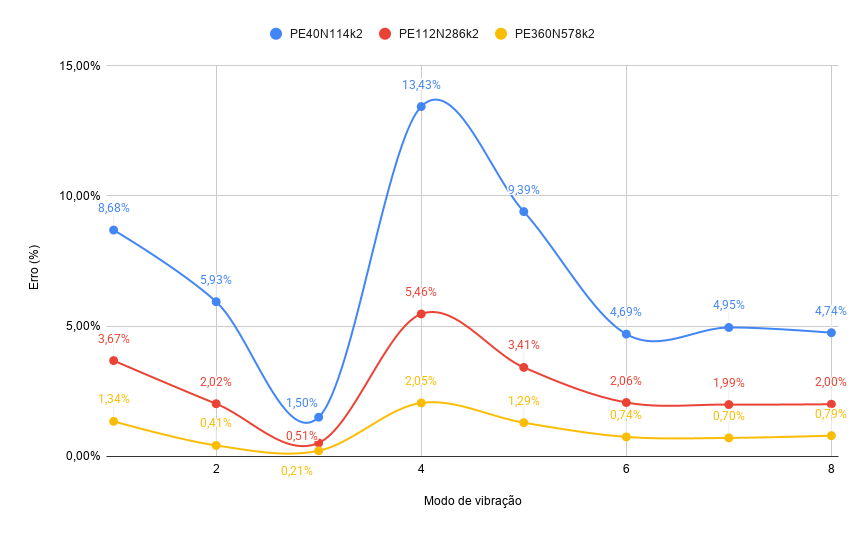
\includegraphics[width=0.9\textwidth]{figuras/Capítulo 5/Parede estrutural/Erros relativos k2-2.png}
    \label{fig:5.20}

    \centerline{{\small \textbf{Fonte:} Elaborado pelo autor (2026).}}
\end{figure}

\indent Comparando as curvas das figuras~\ref{fig:5.19} e \ref{fig:5.20} Nota-se que a divergência dos erros se encontra nos modos de vibração superiores. O parâmetro estabilização de baseado no diâmetro tende a atuar de modo mais restritivo nas maiores frequências ajudando a filtrar os modos artificiais. Nas malhas refinadas, o valor do parâmetro de estabilização tende a zero, o que justifica a equivalência dos erros.\\
\indent Para comparação dos resultados, serão tomados os valores do MEF quadrático e do MEFG de \citet{custodio2022metodo}. Os erros entre os métodos em relação à formulação de referência (A~$\alpha$~FEM) encontram-se na Tabela~\ref{tab:5.22}. \\
\indent Comparando os resultados da tabela, verifica-se que os resultados globais do MEV de alta ordem foram superiores aos do MEF e ao MEFG em todas as malhas para a MAPE, todavia o mesmo resultado não se repete para a NRMSE e a MG, onde o MEV só obteve melhores resultados que os outros dois métodos na malha mais refinada.

% Certifique-se de ter \usepackage{makecell} no preâmbulo do documento.

\begin{table}[htbp]
    \centering
    \caption{Comparação de erros do MEV com o MEF-T6 e MEFG.}
    \label{tab:5.22}
    \small % Reduz o tamanho da fonte para o padrão acadêmico
    \begin{tabular}{lccccc}
        \toprule
        \textbf{Modelo} & 
        \makecell{\textbf{MEF}\\\textbf{(826 gl)}} & 
        \makecell{\textbf{MEFG}\\\textbf{(1152 gl)}} & 
        \textbf{PE40N114k2} & 
        \textbf{PE112N286k2} & 
        \textbf{PE360N262k2} \\
        \midrule
        MAPE  & 14,15\% & 12,67\% & 6,66\% & 2,64\% & 0,94\% \\
        NRMSE & 1,36\%  & 2,22\%  & 6,64\% & 2,65\% & 0,99\% \\
        MG    & 4,38\%  & 5,30\%  & 6,65\% & 2,64\% & 0,96\% \\
        \bottomrule
    \end{tabular}
    
    \vspace{0.2cm}
    \raggedright
    \textbf{Fonte:} Elaborado pelo autor (2026).
\end{table}

\indent Avaliando o ganho de precisão relativo do MEV de alta ordem em relação à malha de elementos finitos quadráticos, para a MAPE, o ganho de discretização apresenta mínimo de 53\% e máximo de 93\%. Ao analisar a NRMSE, com a maior penalização do erro, tanto as malha de 40 quanto a de 112 elementos obtiveram resultados inferiores ao de elementos finitos, com perda de precisão de -389\% na malha mais grosseira. Os resultados da MG por serem a média da MAPE e da NRMSE obteve um ganho de precisão de 40\% apenas para a malha de 112 elementos.

\begin{table}[htbp]
    \centering
    \caption{Ganho de precisão relativo do MEV em relação ao MEF -- Modelos de alta ordem.}
    \label{tab:5.23}
    \small % Reduz o tamanho da fonte para o padrão acadêmico
    \begin{tabular}{lccc}
        \toprule
        \textbf{Modelo} & \textbf{PE40N114k2} & \textbf{PE112N286k2} & \textbf{PE360N578k2} \\
        \midrule
        MAPE  & 53\%   & 81\%  & 93\% \\
        NRMSE & -389\% & -95\% & 27\% \\
        MG    & -52\%  & 40\%  & 78\% \\
        \bottomrule
    \end{tabular}
    
    \vspace{0.2cm}
    \raggedright
    \textbf{Fonte:} Elaborado pelo autor (2026).
\end{table}

\indent Para comparar o ganho de precisão do MEV e do MEFG em relação ao MEF quadrático utilizam-se os coeficientes de acurácia da tabela~\ref{tab:5.23}. Avaliando o CA com base na MG, nota-se que com todas as malhas obtiveram maior acurácia que o MEFG, os resultados negativos ocorrem por que o resultado do MEFG foi inferior ao de elementos finitos quadráticos.

\begin{table}[htbp]
    \centering
    \caption{Coeficientes de acurácia para o problema da parede estrutural com formulação de alta ordem.}
    \label{tab:524}
    \small % Reduz o tamanho da fonte para o padrão acadêmico
    \begin{tabular}{lccc}
        \toprule
        \textbf{Modelo} & \textbf{PE40N114k2} & \textbf{PE112N286k2} & \textbf{PE360N578k2} \\
        \midrule
        MAPE  & 5,07 & 7,80  & 8,95  \\
        NRMSE & 6,17 & 1,51  & -0,43 \\
        MG    & 2,48 & -1,90 & -3,74 \\
        \bottomrule
    \end{tabular}
    
    \vspace{0.2cm}
    \raggedright
    \textbf{Fonte:} Elaborado pelo autor (2026).
\end{table}


\indent Os deslocamentos são comparados aos de \citet{nguyenthanh2010alternative} utilizando a malha PE360N578k2. Os deslocamentos obtidos com o MEV podem ser vistos na Figura~\ref{fig:5.21} enquanto os de \citet{nguyenthanh2010alternative} estão na figura~\ref{fig:5.22}

    \begin{figure}[H]
        \centering
        \caption{Primeiro e oitava modo de vibração do MEV}
        \label{fig:5.21}
        \begin{subfigure}[b]{0.45\textwidth}
            \centering
            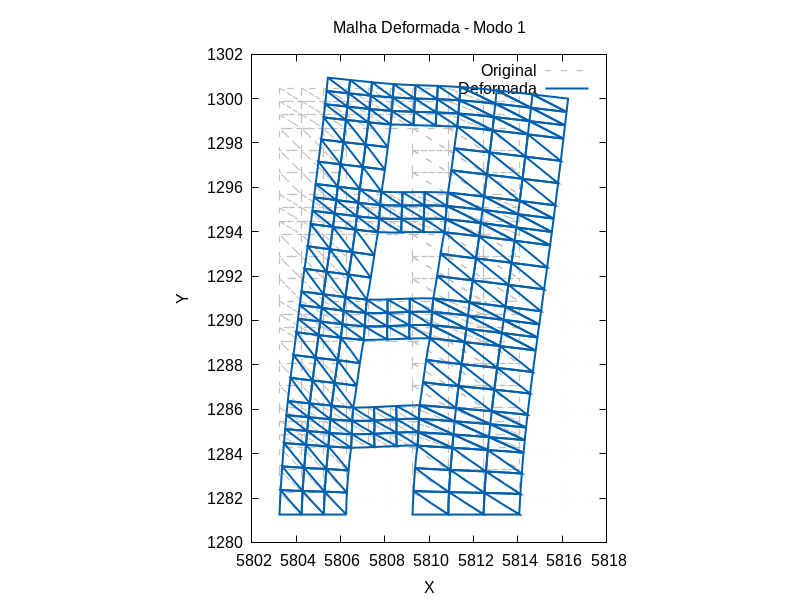
\includegraphics[width=\textwidth]{figuras/Capítulo 5/Parede estrutural/deformed_mode_1.png}
            \label{fig:5.21a}
        \end{subfigure}
        \hfill
        \begin{subfigure}[b]{0.45\textwidth}
            \centering
            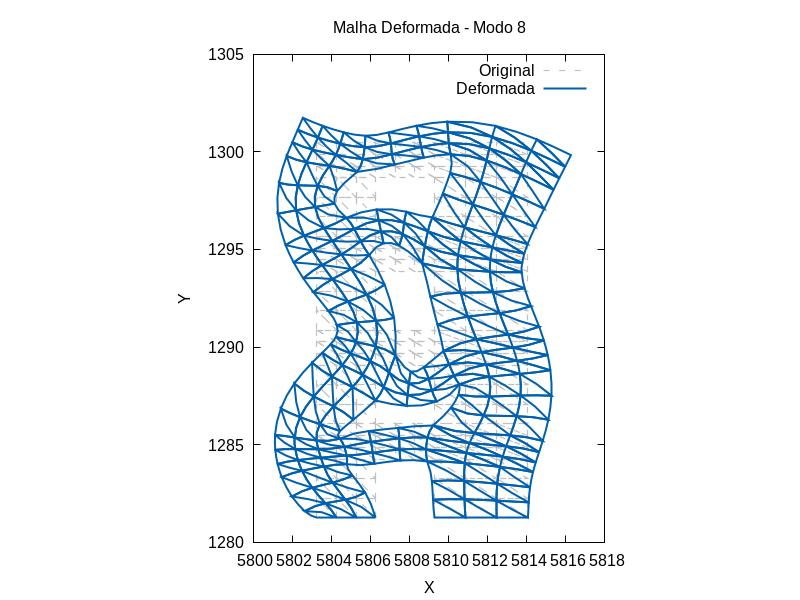
\includegraphics[width=\textwidth]{figuras/Capítulo 5/Parede estrutural/deformed_mode_8.png}
            \label{fig:5.21b}
        \end{subfigure}

        \centerline{        {\small \textbf{Fonte:} Elaborado pelo autor (2026).}}
    \end{figure} 

        \begin{figure}[H]
        \centering
        \caption{Primeiro e oitavo modo de vibração de \citet{nguyenthanh2010alternative}}
        \label{fig:5.22}
        \begin{subfigure}[b]{0.45\textwidth}
            \centering
            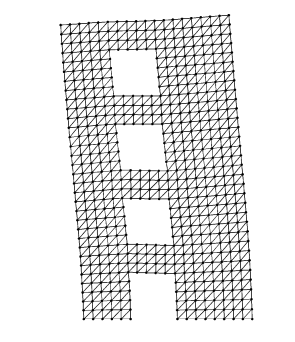
\includegraphics[width=.5\textwidth]{figuras/Capítulo 5/Parede estrutural/Captura de tela 2026-09-16 084739.png}
            \label{fig:5.22a}
        \end{subfigure}
        \hfill
        \begin{subfigure}[b]{0.45\textwidth}
            \centering
            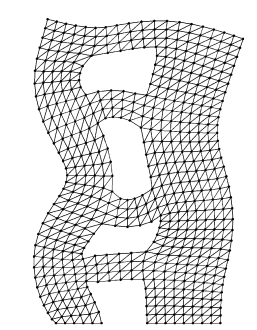
\includegraphics[width=0.5\textwidth]{figuras/Capítulo 5/Parede estrutural/Captura de tela 2026-09-16 084801.png}
            \label{fig:5.22b}
        \end{subfigure}

        \centerline{        {\small \textbf{Fonte:} \citet{nguyenthanh2010alternative}.}}
    \end{figure} 



\indent Com o refino-p, foi feito um estudo sobre o comportamento do condicionamento das matrizes de rigidez e massa na solução. As figura~\ref{fig:5.23} apresenta os valores do número de condicionamento das matrizes de massa e rigidez para o caso $k=2$. Como pode ser notado, ao comparar com a figura~\ref{fig:5.26}, o número de condicionamento das matrizes de cresceram com um fator de $x100$ ao realizar o refino-p.

\begin{figure}[H]
        \centering
        \caption{Primeiro e oitava modo de vibração do MEV}
        \label{fig:5.21}
        \begin{subfigure}[b]{0.45\textwidth}
            \centering
            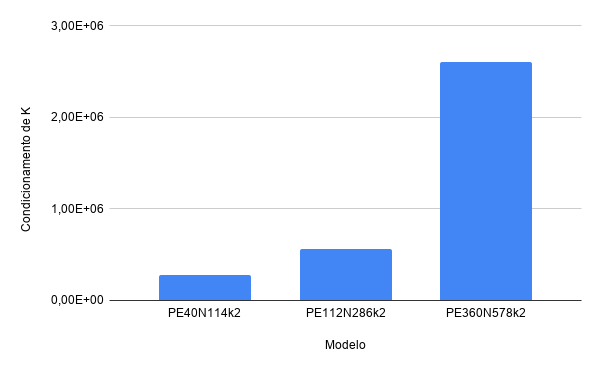
\includegraphics[width=\textwidth]{figuras/Capítulo 5/Parede estrutural/Condicionamento de K 2.png}
            \label{fig:5.21a}
        \end{subfigure}
        \hfill
        \begin{subfigure}[b]{0.45\textwidth}
            \centering
            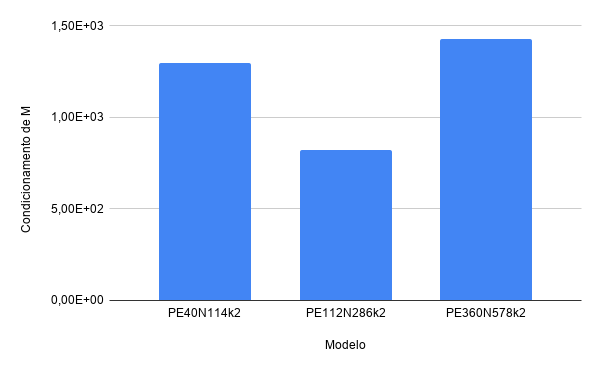
\includegraphics[width=\textwidth]{figuras/Capítulo 5/Parede estrutural/Condicionamento de M 2.png}
            \label{fig:5.21b}
        \end{subfigure}

        \centerline{        {\small \textbf{Fonte:} Elaborado pelo autor (2026).}}
    \end{figure} 

\indent Como asseverado por \citet{illconditioningvirtualelementmethodstabilizationsbases2018}, os graus de liberdade internos possuem um peso muito maior no condicionamento da matriz de rigidez do que as diversas estabilizações, expondo que os monômios escalados utilizados tradicionalmente na literatura implicam em um aumento exponencial do número de condicionamento em termos de $k$. Fato que pode ser verificado através da Figura~\ref{fig:5.30}. Uma forma de combater esse efeito é o emprego da base canônica ortonormal, que pode ser construída através do algoritmo de Gram-Schmidt. \\
\indent Ao avaliar a relação do tempo de solução com o tempo de execução na figura~\ref{fig:5.33} percebe-se que o tempo de solução não apresenta relação com os valores do número de condicionamento do modelo. A grande parte dos modelos se encontra perto de 1 segundo com algumas exceções perto dos 4 segundos. Os resultados levem a entender que existe uma relação maior entre o tempo de solução do que com o número de condicionamento das matrizes de massa e rigidez.

\begin{figure}[H]
    \centering
    \caption{Relação entre o número de condicionamento e o tempo de execução.}
    \label{fig:5.33}
    \begin{subfigure}[b]{\textwidth}
        \centering
        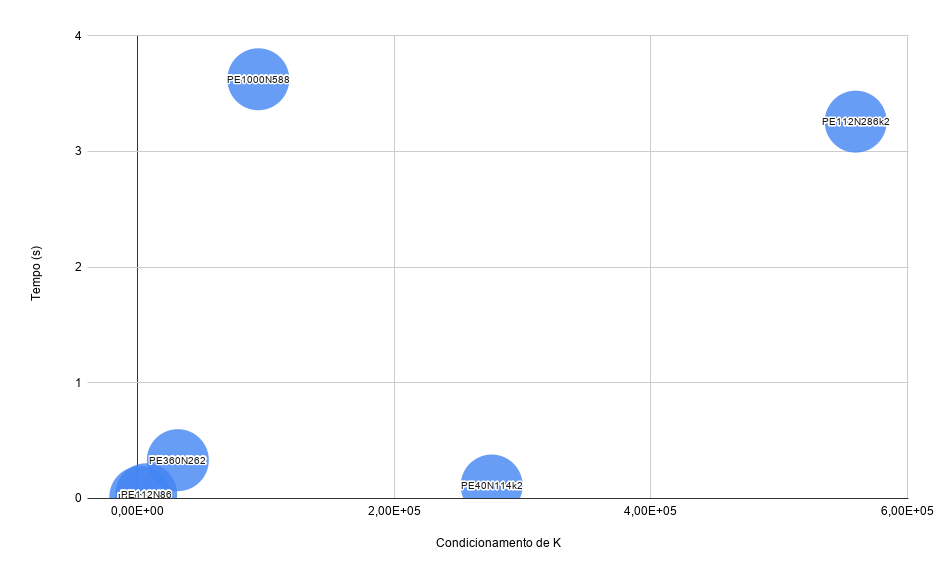
\includegraphics[width=\textwidth]{figuras/Capítulo 5/Parede estrutural/TxCond - K.png}
        \label{fig:5.32a}
    \end{subfigure}
    
    \begin{subfigure}[b]{\textwidth}
        \centering
        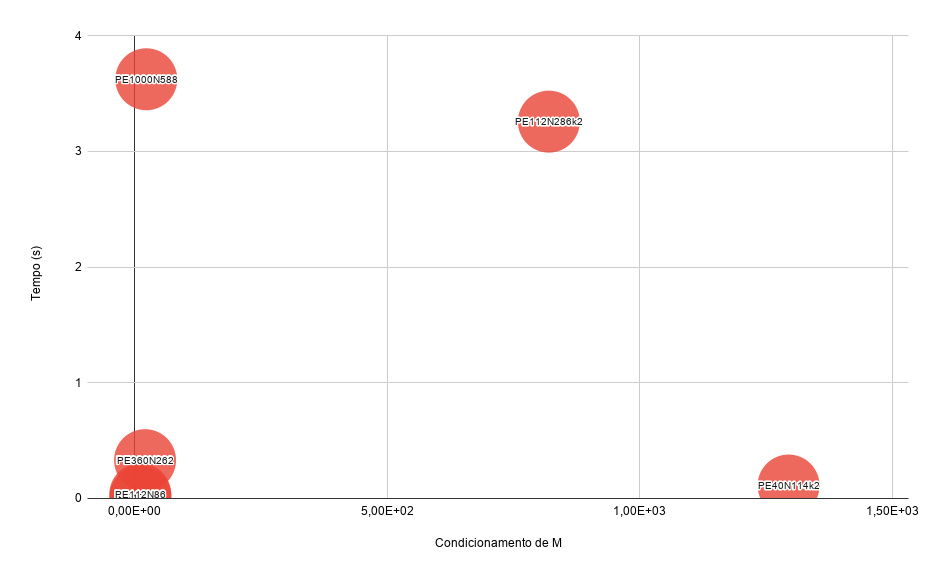
\includegraphics[width=\textwidth]{figuras/Capítulo 5/Parede estrutural/TxCond - M.png}
        \label{fig:5.32b}
    \end{subfigure}

    \centerline{{\small \textbf{Fonte:} Elaborado pelo autor (2026).}}
\end{figure}


\indent Em relação ao tempo de execução, nota-se pela Figura~\ref{fig:5.32} que, apesar de a quantidade de elementos estar, sim, relacionada ao tempo de processamento, o grau de aproximação possui também possui impacto no tempo, o que pode ser explicado pela quantidade adicional de graus de liberdade. Observa-se-se que o tempo de montagem dos elementos é muito mais curto do que o tempo de solução do sistema. 

\begin{figure}[H]
    \centering
    \caption{Tempo de execução em função da quantidade de elementos.}
    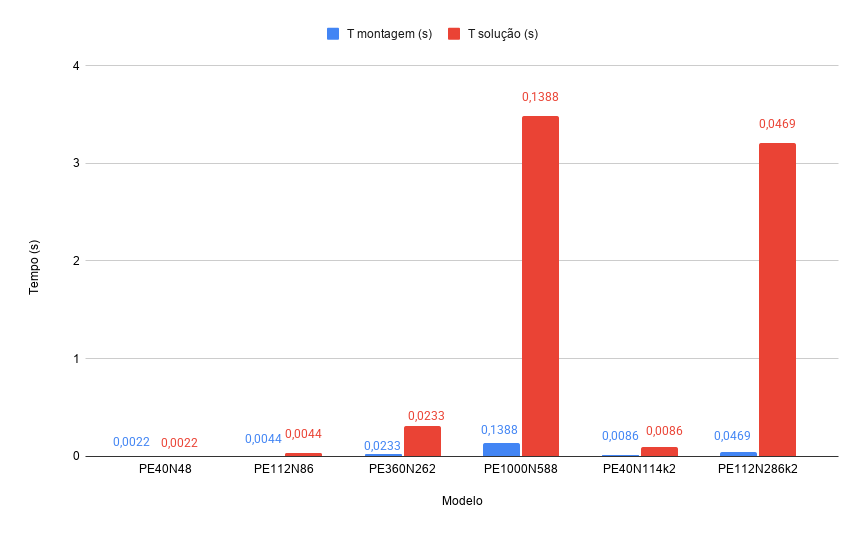
\includegraphics[width=\textwidth]{figuras/Capítulo 5/Parede estrutural/TxElementos.png}
    \label{fig:5.32}

    \centerline{    {\small \textbf{Fonte:} Elaborado pelo autor (2026).}}
\end{figure} 

